\documentclass[a4paper,11pt,oneside]{book}

% packages 
\usepackage{arsclassica}    % fancy layout
\usepackage[english]{babel}\addto{\captionsenglish}{\renewcommand{\bibname}{References}}
\usepackage{caption}         % figure captions
\usepackage[square,numbers,super,sort&compress]{natbib}  % bibliography style
\usepackage[cc]{titlepic}    % enable logo on title page
\usepackage{graphicx}       % logo related

% Margins for pretty version ::
%\usepackage[pass]{geometry}
% Margins for university regulations ::
\usepackage[top=2cm, bottom=4cm, left=4cm, right=2.5cm]{geometry}
\usepackage{setspace}
\onehalfspacing

\usepackage{standalone}
\standalonetrue

% don't hang captions
\captionsetup{format=plain}

% bibliography
\bibliographystyle{../thesis}

% title setup
\title{ \vspace{3in} Unravelling higher order genome organisation {\small [working
    title]} \\ \vspace{2em} {\large {\bf Results 3: Domain boundaries}} }
\author{Benjamin L. Moore}
\titlepic{\vspace{2.2in} 
\includegraphics[width=\textwidth]{/Users/benmoore/hvl/1yrReport/figs/igmm.png}}

\begin{document}

%\maketitle

\chapter{Chromatin domain boundaries}\label{chap:boundaries}

\section{Introduction}

Multiple studies have defined chromatin domains of different types, for example: chromosome compartments;\cite{Lieberman2009} topological associating domains (TADs);\cite{Dixon2012} contact and loop domains;\cite{Rao2014} physical domains;\cite{Sexton2012, Hou2012} and others.\cite{Filippova2014} The existence of these domains necessitates "boundary regions" either between consecutive domains or bookending more sparsely-positioned domains, however the functional relevance of said boundary regions is still open to debate.

In their study of topological domains, Dixon \emph{et al.} identified average enrichments over TAD boundary regions in both human and mouse for various features including CTCF and PolII.\cite{Dixon2012} Boundaries were also enriched for signs of active transcription, such as with the histone modification H3k36me3. These results, coupled with an observable enrichment for promoters at domain boundaries, have lead to the theory that boundaries may act as an additional layer of transcriptional control,\cite{Sexton2015} however an alternative theory could be that looping between enhancer elements and promoters results in an observable boundary through C-method experiments.\cite{Rao2014} Another non-exclusive explanation is that if chromatin domains represent co-regulatory regions as is widely thought,\cite{LeDily2014, Nora2013, Sexton2015} boundaries themselves could be mere side-effects and as such of limited biological interest.

An obvious experiment to resolve these opposing theories would be to delete a predicted boundary region and test for local changes in both contacts and expression. Such an experiment was performed on a region of the human X-chromosome containing the genes encoding the dosage-compensation long non-coding RNAs Xist and Tsix, which are separated by a TAD boundary.\cite{Nora2012} This study found that while histone modifications within the body of a TAD could be removed without affecting the structure, deletion of a boundary did have an effect and lead to increased intradomain contacts.\cite{Nora2012} Surpsingingly however, this effect was not total and some observable barrier remained, lending evidence that TADs may be centrally constrained, rather than by their borders.\cite{Nora2012} 

A second experiment used CRISPR genome editing to link TAD boundary changes with limb development disorders,\cite{Lupianez2015} indicating that boundary changes could provide an underlying explanation for pathogenic non-coding structural variants.\cite{Ren2015} Similarly, domain boundaries on X-chromosomes were found to be weakened following the disruption of condensation binding sites.\cite{Crane2015} Together these studies suggest a complex scenario whereby TAD boundaries are an important structural feature, yet do not fully explain domain partitioning.

Computational analysis of boundaries has emerged during the time this work was completed. Border "strength", here defined by the ratio of total intra:inter-domain contacts, was found to correlate with increased occupancy of a combination of bound architectural proteins.\cite{VanBortle2014}

Many questions remain about chromatin boundaries. For example, are the observed enrichments persistent across cell types and how do they compare across organisation strata, such as compartments and TADs? Through computational analysis of the set of boundaries re-called from published datasets, we can investigate these questions and probe boundary enrichments across a broad array of locus-level chromatin features.

\section{TAD and compartment boundaries}\label{sec:boundaryenrichments}

The mammalian genome is organized into TADs, predominantly self-interacting chromatin domains, with boundary regions reportedly associated with pronounced peaks and troughs of particular features within 500 kb of the predicted boundary.\cite{Dixon2012} Exploration of this phenomenon using a set of 24 mouse ESC chromatin features (and a smaller number of human ESC features) reportedly revealed enrichment peaks of CTCF, H3K4me3 and H3K36me3, as well as a pronounced dip in H3K9me3, suggesting that high levels of transcription may contribute to boundary formation.\cite{Dixon2012} However, it was unclear whether other features show unusual patterns in TAD boundary regions, and whether the constellation of features involved changes between cell types. The features associated with boundaries separating A and B compartments calculated from Hi-C eigenvectors have not been studied to our knowledge. The datasets assembled here, consisting of 35 matched chromatin features across three cell types, allow us to conduct the first comparative study of the constituents of human TAD and compartment boundary regions.

We derived TAD boundaries according to established methods (see Methods \ref{meth:tadcalling}) for all three cell types under study. We then sought evidence for significantly enriched or depleted features at TAD boundary regions using a conservative approach (a nonparametric statistical test and Bonferroni multiple testing correction, see Methods \ref{tads}).

\begin{figure}
\begin{center} 
\makebox[\textwidth][c]{ 
	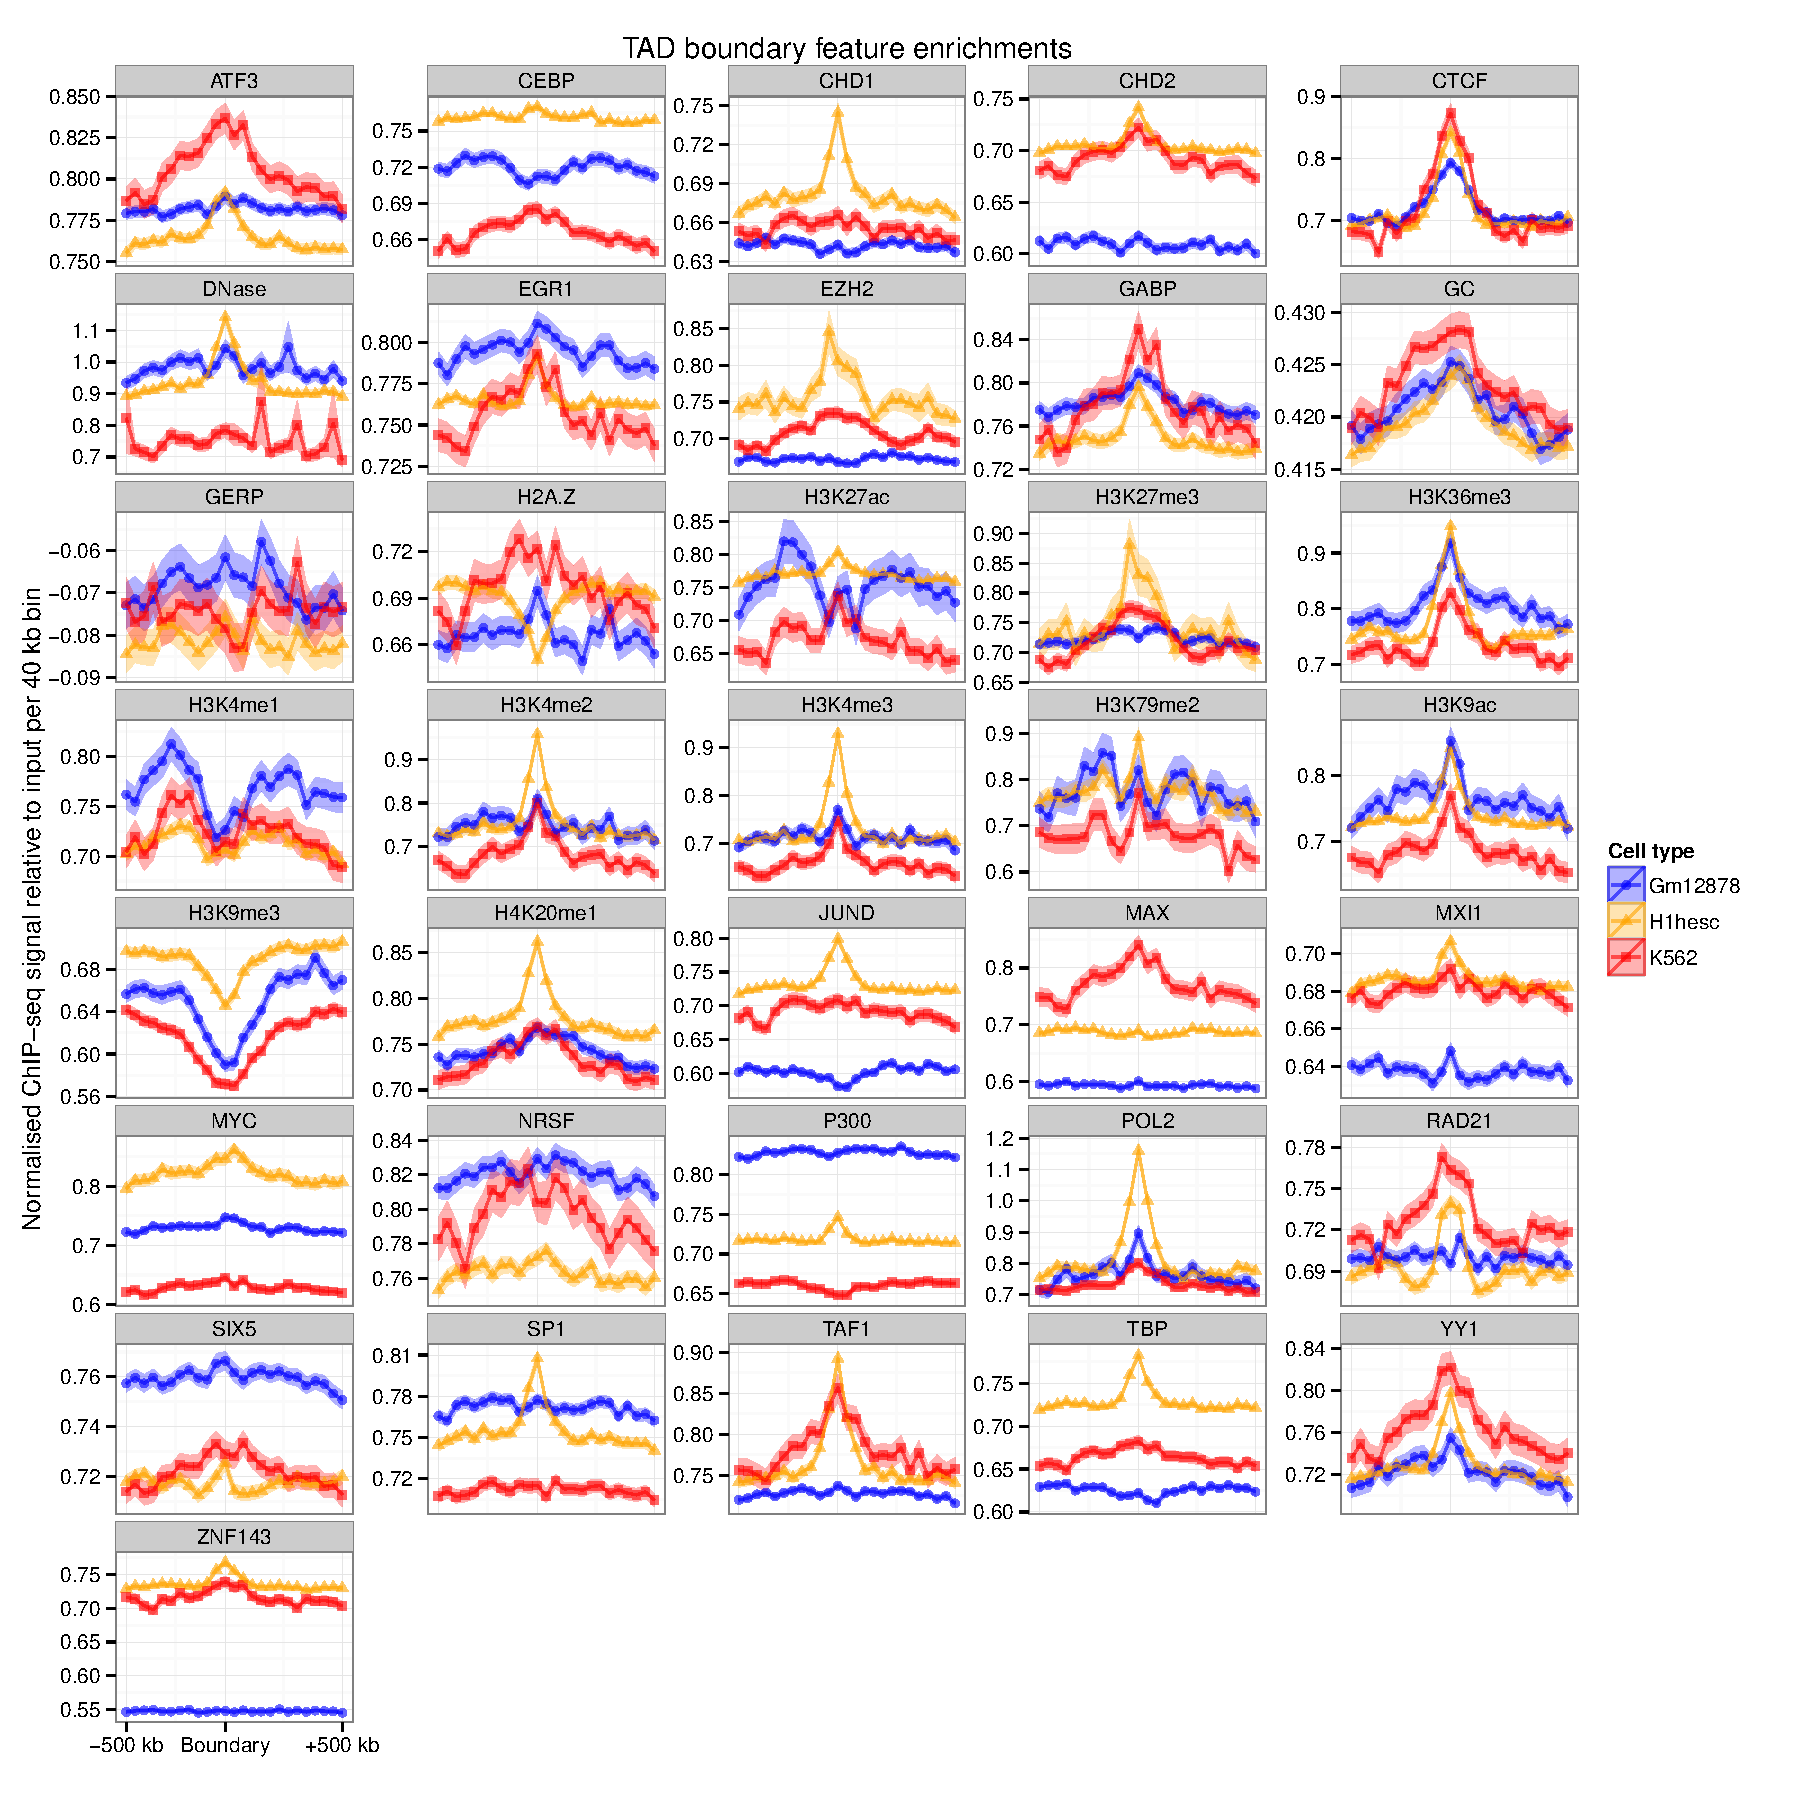
\includegraphics[width=6.8in]{figs/alltads.pdf}
}
\captionsetup{width=\textwidth}
\caption[TAD boundary enrichments and depletions.]{ {\bf TAD boundary enrichments and depletions.}
36 features were averaged over 1 Mb windows centred on TAD boundaries genome-wide ($25 \times 40$ kb bins). Ribbons represent $95\%$ confidence intervals of the mean at each position.
}\label{fig:alltads}
\end{center}
\end{figure} 

\begin{figure}
\begin{center} 
\makebox[\textwidth][c]{ 
	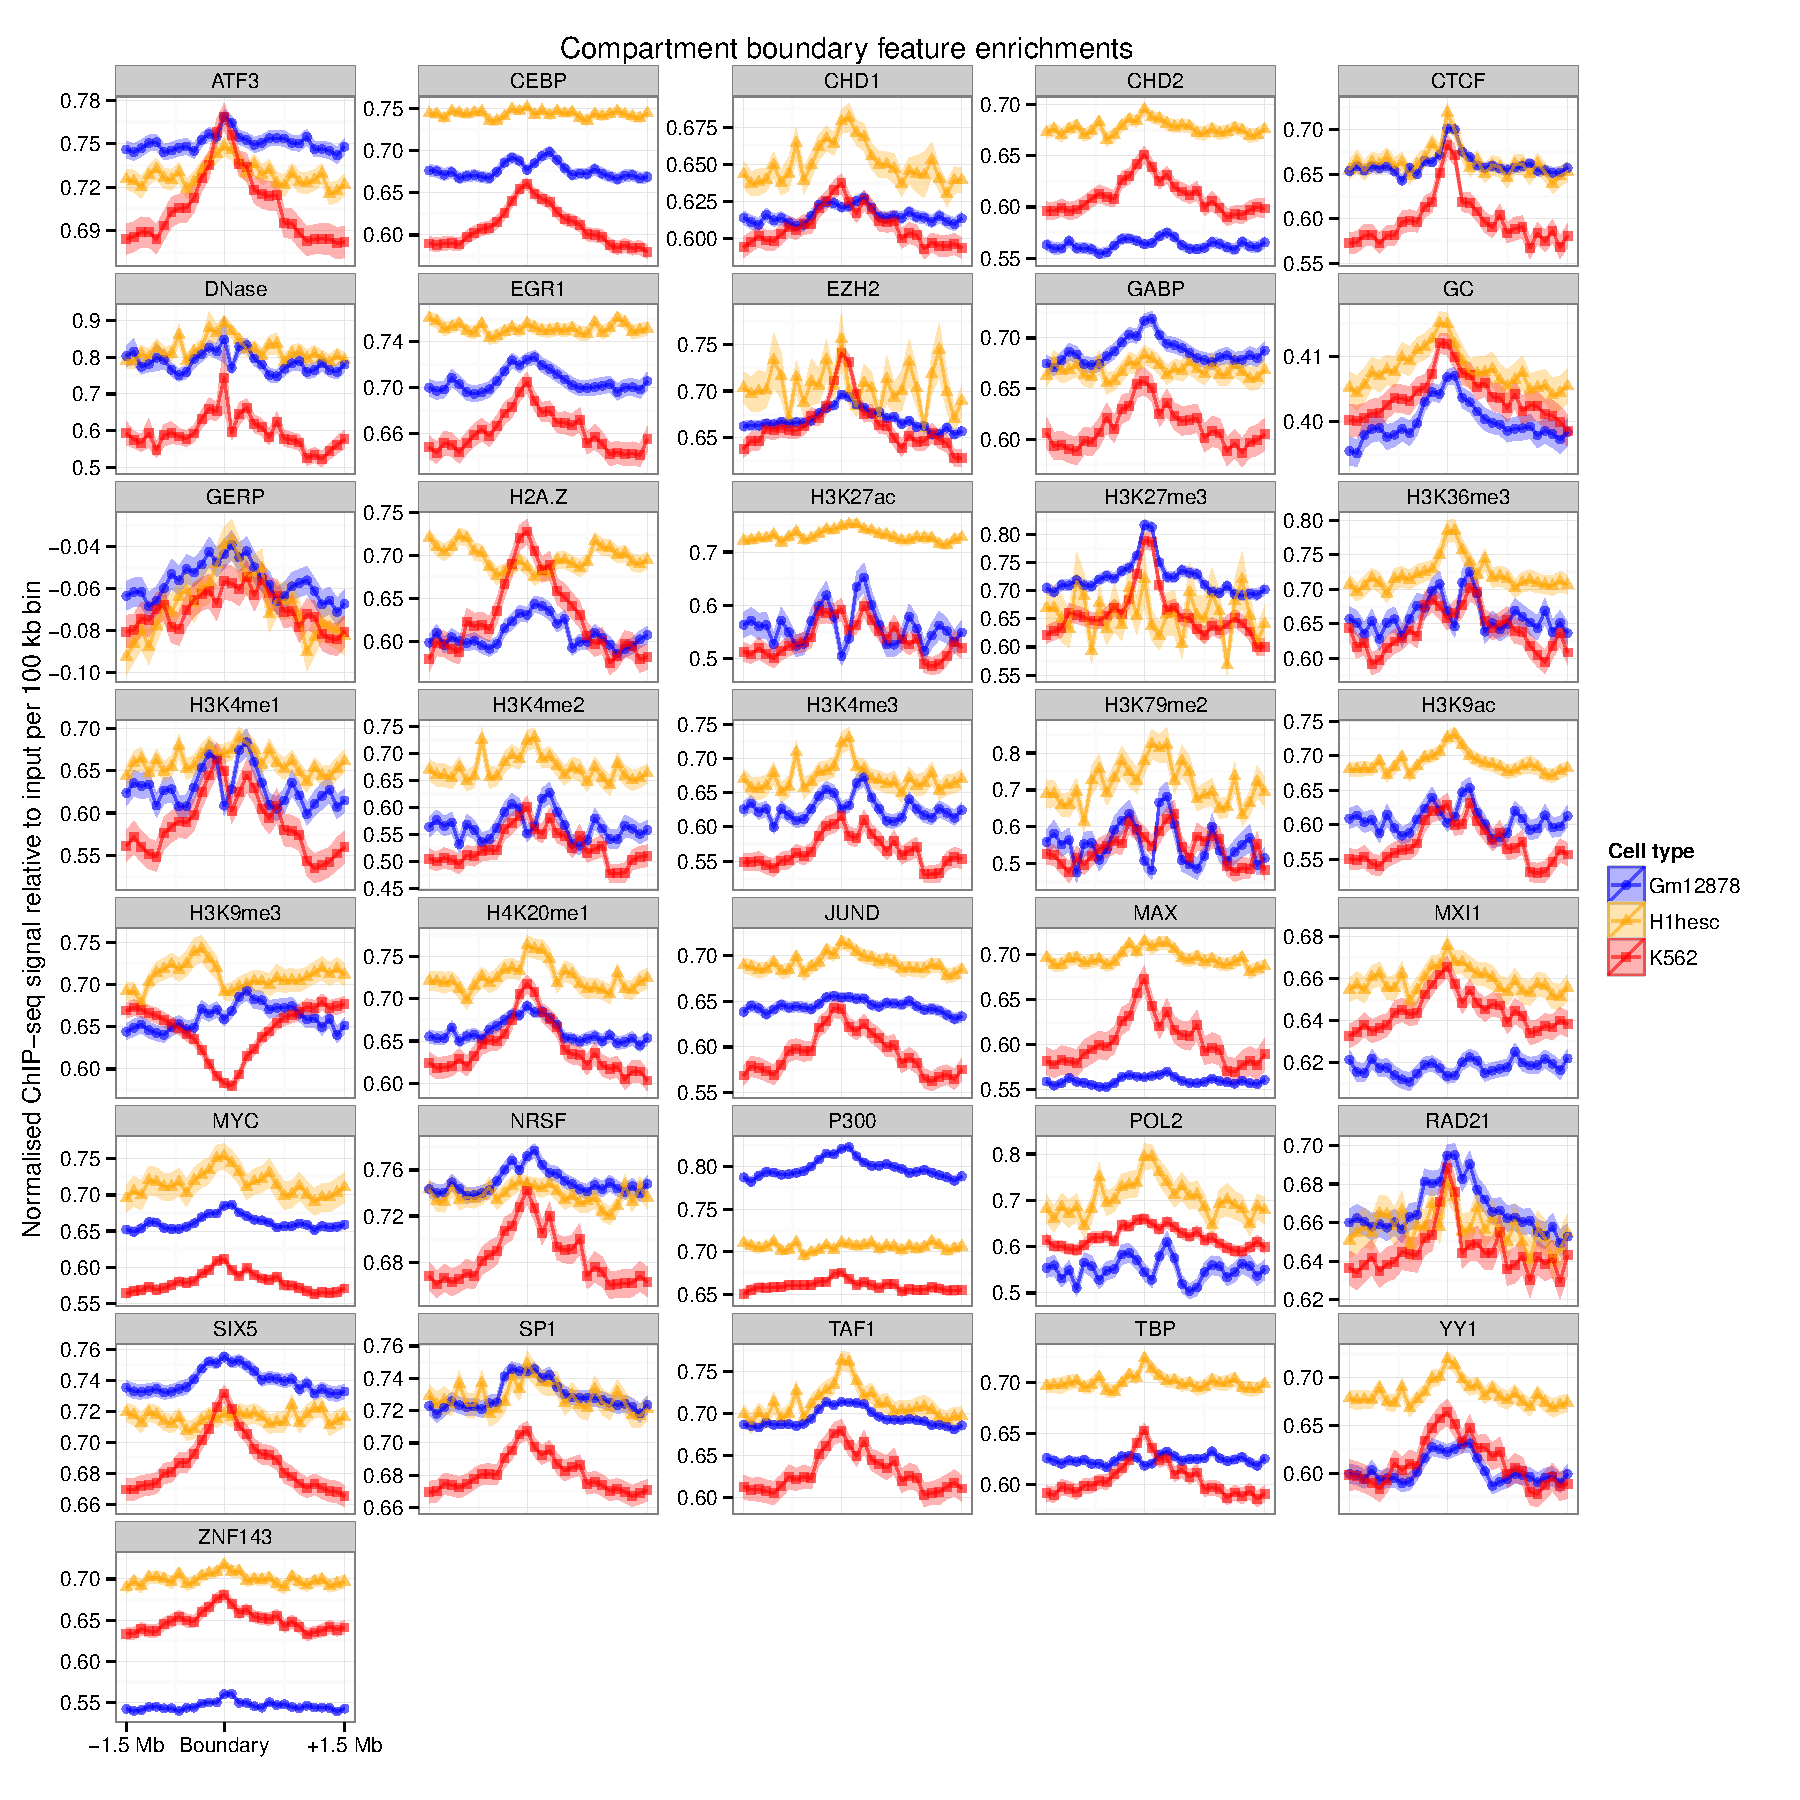
\includegraphics[width=6.8in]{figs/allcompartments.pdf}
}
\captionsetup{width=\textwidth}
\caption[Compartment boundary enrichments and depletions.]{ {\bf Compartment boundary enrichments and depletions.}
36 features were averaged over 3 Mb windows centred on compartment boundaries genome-wide ($30 \times 100$ kb bins). Ribbons represent $95\%$ confidence intervals of the mean at each position.
}\label{fig:allcompartments}
\end{center}
\end{figure} 

Our findings confirmed the previously reported peaks (CTCF and POL2) and dip (H3K9me3) in ESC data, but also revealed substantial heterogeneity between cell types. CTCF binding was found enriched at TAD boundaries across all cell types, but other features, including H3K36me3 and H3K4me3, show dramatic peaks of enrichment in H1 hESC cells that are not seen consistently in other cell types (Figure 6, Additional file 1: Figure S12). Although the dip in H3K9me3 at TAD boundaries is seen in all cell types, the extent of the depletion varies and is weakest in H1 hESC cells. Many other features show significant, though often modest, enrichments in a particular cell type. However, overall the complexity of TAD boundaries (measured as the number of strongly enriched features) is notably higher in H1 hESC than in the other two, more differentiated, cell types (Figure 6), involving large increases in the binding of sequence specific factors such as SP1 and JUND.

\begin{figure}
\begin{center} 
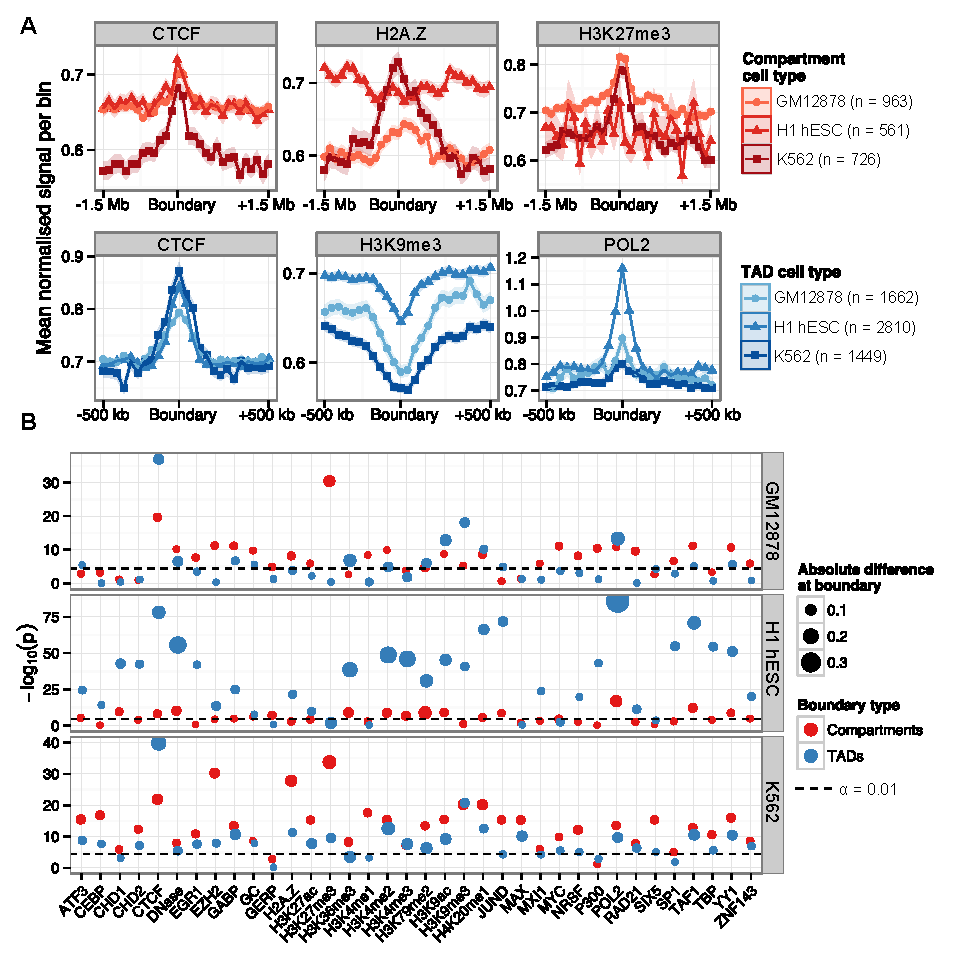
\includegraphics[width=5.5in]{figs/boundarysummary.pdf}
\captionsetup{width=\textwidth}
\caption[Compartment and TAD boundary enrichment summary in three human cell types.]{ {\bf Compartment and TAD boundary enrichment summary in three human cell types.}
(A) Selected profiles for locus-level features are shown for TAD boundaries (CTCF, H3K9me3 and POL2) and compartment boundaries (H2A.Z, H3K4me2 and YY1), as a mean normalized ChIP-seq signal relative to input chromatin per bin ($\pm1$ standard error). TAD boundaries were examined over $40$ kb bins over the $1$ Mb flanking each boundary; compartment boundaries were examined over 100-kb bins over $3$ Mb. (B) The significance of enrichment or depletion ($-\log_{10}(p)$ two-tailed Mann--Whitney test) of a feature was calculated as the boundary bin relative to the ten most peripheral bins (five either side). Points are scaled by the absolute mean difference in signal over the boundary relative to the mean of peripheral bins. ChIP-seq, chromatin immunoprecipitation sequencing; TAD, topological domain.
}\label{fig:boundarysummary}
\end{center}
\end{figure} 

Across all three cell types several features demonstrate consistent
and statistically significant patterns at TAD boundaries (Figure 6,
Figure S12), including peaks associated with active transcription of
genes (POL2, H3K9ac) and dips in H3K9me3, as previously reported.\cite{Dixon2012} However other novel feature peaks of interest emerge
across cell types, such as peaks of H4K20me1, a modification
previously implicated in chromatin compaction.\cite{Evertts2013} We also observe consistent increases in GC content at TAD boundaries, at a scale that is difficult to reconcile with the presence of smaller-scale features such as repeat elements or CpG islands (Additional file 1: Figure S12).

Where neighbouring genomic regions occupy contrasting A and B nuclear
compartments, the disparity implies the presence of a boundary
region. Putative compartment boundaries were identified by using an
HMM to infer the state sequence of A/B compartments across the genome
based on observed principal component eigenvectors. Analogously to the
TAD boundary analysis we then sought significant enrichments or
depletions in 36 chromatin features over these compartment boundaries
(Figure 6, Figure S13).  Compartment boundaries display similar
spectra of enrichments to previously studied TAD boundaries
\cite{Dixon2012} but at lower resolution, reflecting the different
scales of these levels of organization (Figure 6B, Figure S13). Peaks
associated with active promoters (POL2, TAF1, H3K9ac) are again
evident. Parallel enrichments of CTCF, YY1 and H4K20me1 are also seen
at compartment boundaries, as they were for TAD boundaries, in each
cell type under study. In addition, compartment boundaries show
enrichments of H3K79me2, which is known to play critical roles in
cellular reprogramming.\cite{Onder2012} Remarkably, H3K79me2 has
also recently been shown to mark the borders of small (hundreds of bp)
regions of open chromatin.\cite{Chai2013} Thus there may be
similarities in chromatin compaction boundaries at very different
scales.

Certain features show intriguing contrasts between cell types the
histone variant H2A.Z lacks any trace of enrichment at H1 hESC
compartment boundaries, but is significantly enriched in the other two
cell types (Figure 6A), consistent with reports describing H2A.Z
relocation during cellular differentiation.\cite{Ku2012} Compartment
boundaries also show enrichment for the cohesin complex subunit RAD21
in the two hematopoietic cell types , and cohesin is
another factor implicated in modulating nuclear architecture in
partnership with CTCF.\cite{Zuin2013} Various other enrichments
with very modest effect sizes are also evident at compartment
boundaries (Figure 6B, Figure S13). In contrast to TAD boundaries, the
composition of compartment boundaries appears least complex in H1
hESC, relative to the other two cell types. Overall compartment and
TAD boundaries are associated with overlapping spectra of chromatin
features across cell types. These involve DNA binding proteins
implicated in chromosome architecture (CTCF, YY1, RAD21), but also
implicate the initiation and repression of transcription as critical
to boundary formation. However these two boundary classes occur at
different scales, with patterns of informative features typically
spanning regions up to 500 Kb for TAD boundaries, and patterns
associated with compartment boundaries often spanning more than 1 Mb.

\subsection{CTCF and YY1}

\begin{figure}
\begin{center} 
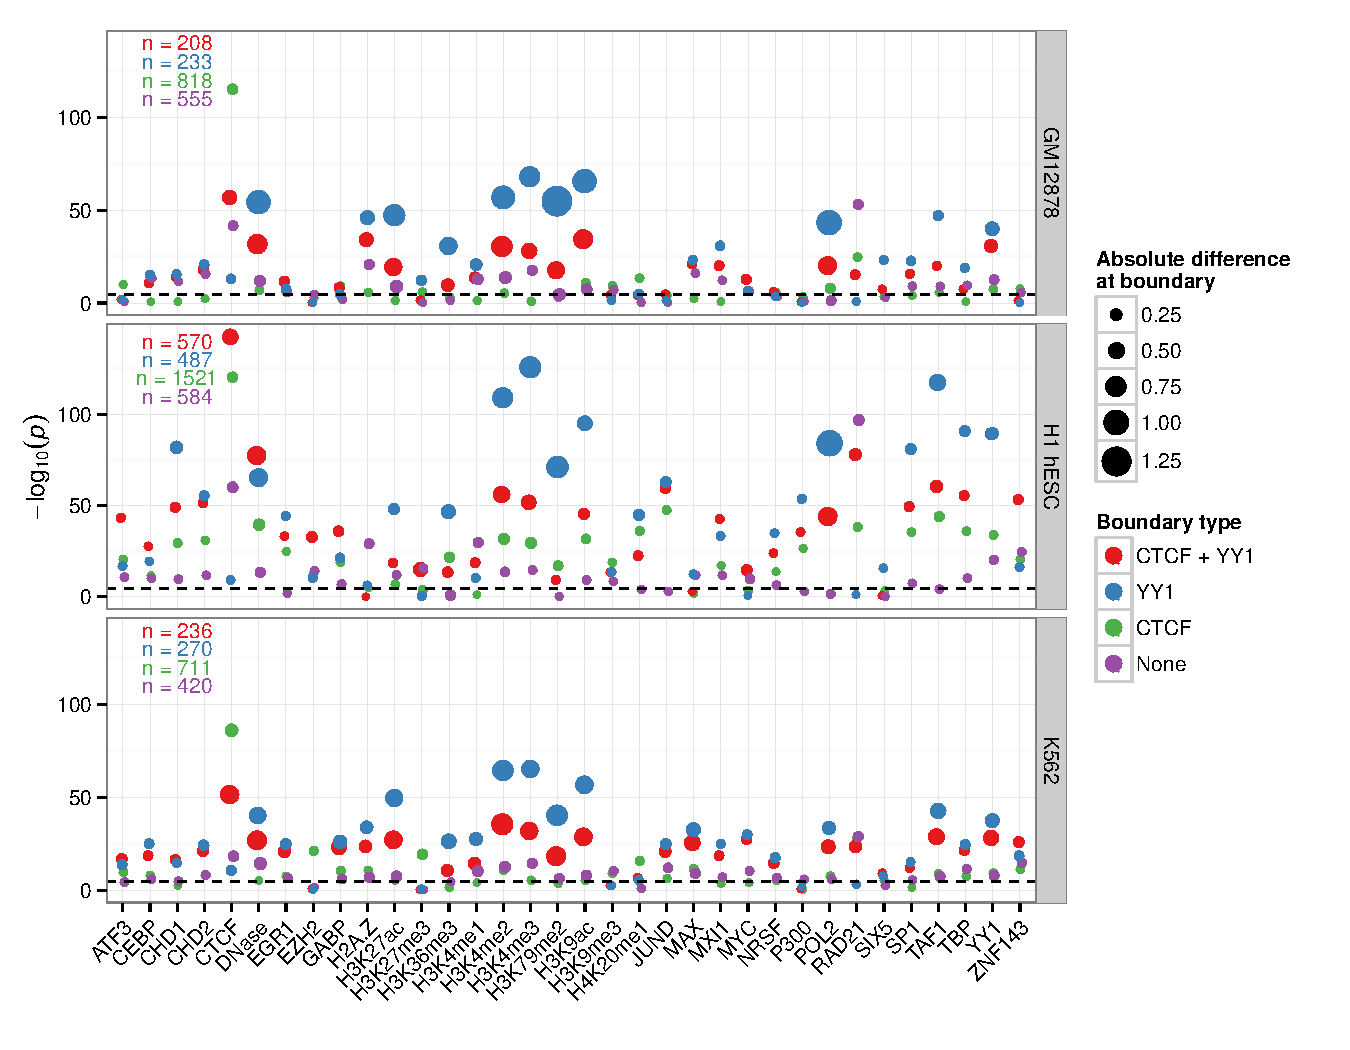
\includegraphics[width=5.8in]{figs/ctcfyy1.pdf}
\captionsetup{width=\textwidth}
\caption[Distinct enrichments of CTCF and YY1 boundaries.]{ {\bf Distinct enrichments of CTCF and YY1 boundaries.}
TAD boundary feature enrichments are shown (as in Fig. \ref{fig:boundarysummary}) for boundaries
split into classes based on specific enrichments: CTCF and YY1 groups are
those boundaries with at least one ENCODE region peak\cite{Dunham2012} for
their respective features, while CTCF + YY1 is the group of boundaries which had one or more
overlapping peaks for these two factors. Boundaries in the �none� group has neither
a CTCF or YY1 region peak called (but can still
be enriched for their respective features in terms of raw signal). 
}\label{fig:ctcfyy1}
\end{center}
\end{figure} 

Significant peaks in YY1 are evident in all cell
types, which is intriguing given the evidence that YY1 and CTCF
cooperate to affect long distance interactions.\cite{Atchison2014} Co-binding of CTCF with YY1 has also been shown
to identify a subset of highly conserved CTCF sites.\cite{Schwalie2013} Co-binding of CTCF and YY1 may also therefore be
a contributing factor in the establishment of TAD boundaries, which
appear to be broadly conserved across mammals.\cite{Dixon2012} To
test this, we split our sets of TAD boundaries into those possessing
ChiP-seq peaks (region peaks called by ENCODE \cite{Dunham2012}) for
CTCF, YY1, both CTCF and YY1 (overlapping peaks) and neither. We then
tested each boundary subset for genome-wide enrichments of the other
features in our dataset (Figure S14). Unexpectedly, we found that
boundaries marked by YY1 (without overlapping CTCF peaks) were
generally most strongly-enriched for other features in our dataset. We
also found that boundaries lacking both CTCF and YY1 peaks showed
instead the strongest enrichments for RAD21 in each cell type (Figure
S14), reinforcing previous findings that describe the distinct
influences of CTCF and cohesin in organizing chromatin structure.\cite{Zuin2013, Seitan2013, Phillips-Cremins2013}

% Schwalie: These observations suggest that with respect to transcriptional activity, YY1 is the functionally dominant factor at co-bound locations.

\subsection{Repeats}\label{sec:repeats}

Dixon \emph{et al}.'s study of TAD boundaries identified short interspersed element (SINE) repeats as being enriched over domain boundaries and suggested roles for these repeats in altering genome organisation, in line with prior evidence.\cite{Dixon2012, Lunyak2007} Interestingly, SINE elements are thought to be responsible for spreading CTCF binding sites through mammalian genomes\cite{Schmidt2012} (thought not in primates\cite{Schwalie2013}). Analysis of recent high-resolution Hi-C data again reported a SINE B2 link with CTCF loops in mice.\cite{Rao2014} Together these results suggest repeats could be a key component in the makeup of domain boundaries.

To investigate this, we used the \texttt{RepeatMasker}\cite{Tarailo-Graovac2009} software package to call repeat classes and families in the \texttt{hg19} and \texttt{mm10} genome assemblies. Counts for each annotated feature were then average over boundaries as described previously (Methods \ref{boundaries}).

\begin{figure}
\begin{center} 
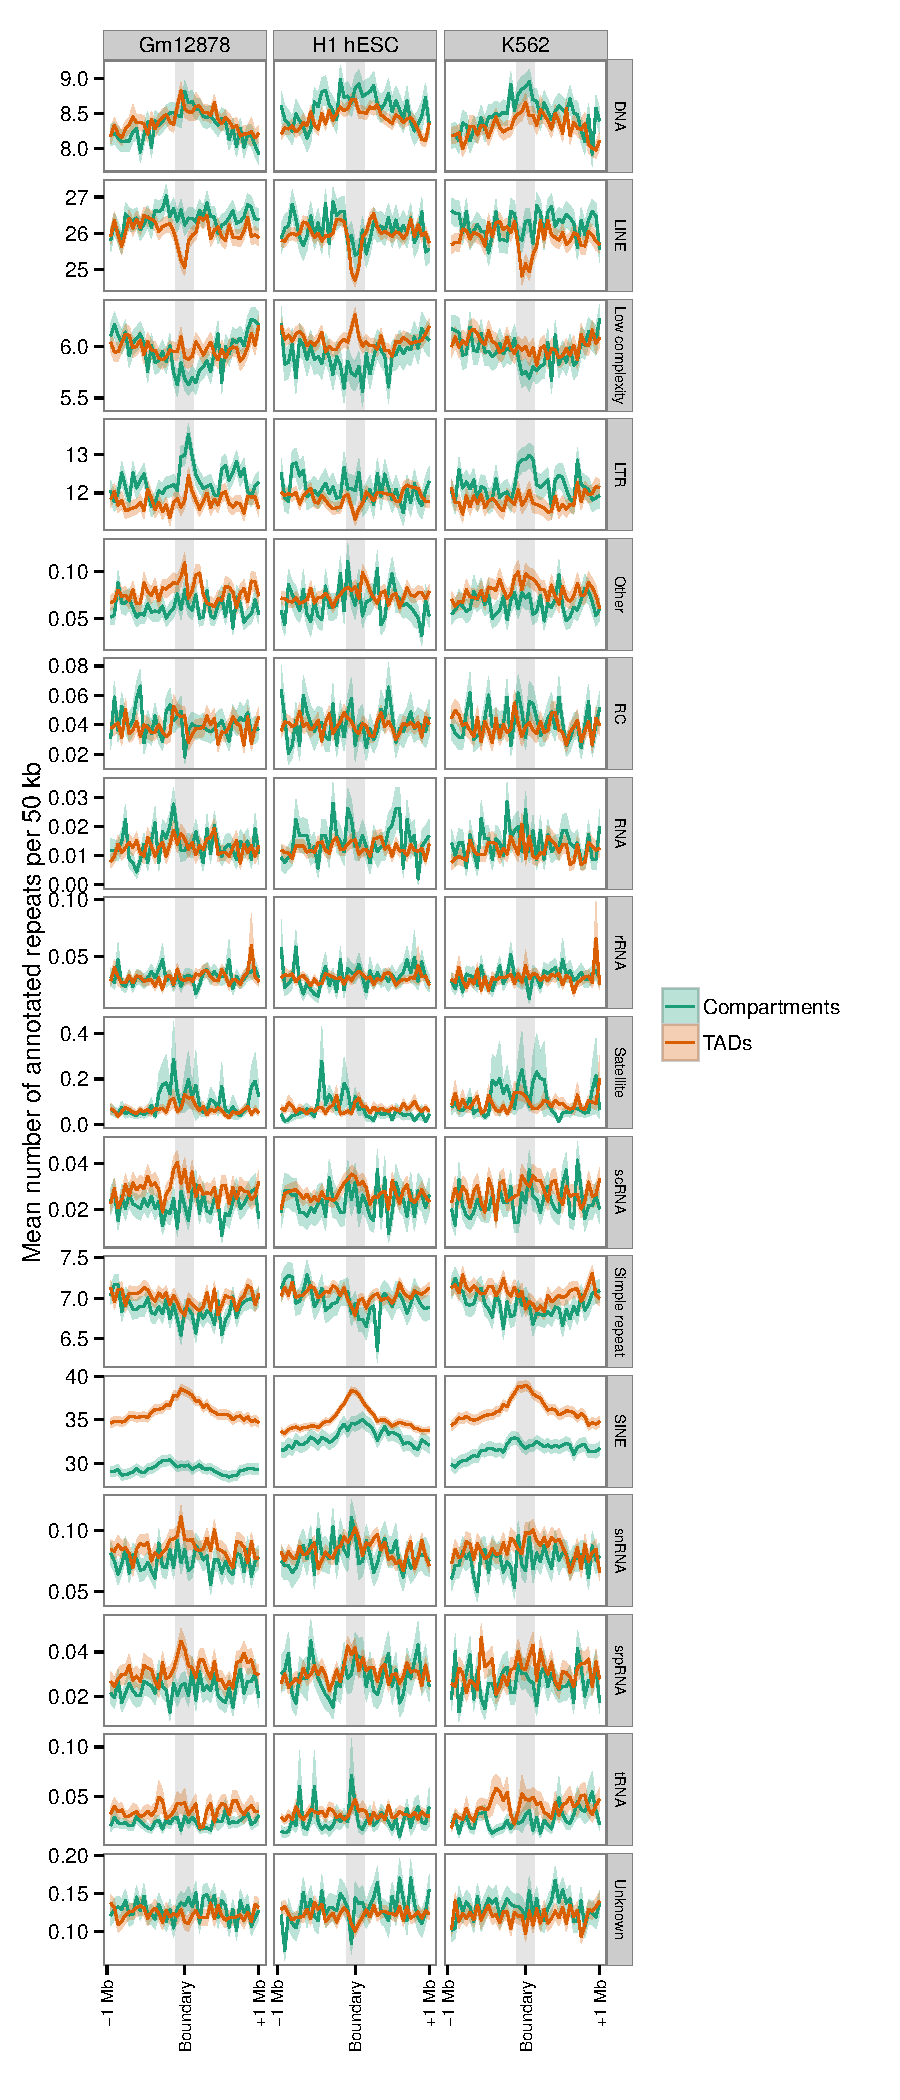
\includegraphics[width=4in]{figs/rep_classprofiles.pdf}
\captionsetup{width=\textwidth}
\caption[Repeat class average-o-grams over all TAD and compartment boundaries.]{ {\bf Repeat class average-o-grams over all TAD and compartment boundaries.}
RepeatMasker repeat annotations are counted per 50 kb for 1 Mb either side of each TAD and compartment boundaries. The mean count genome-wide is plotted with $\pm 95\%$ confidence intervals.
}\label{fig:rep_classprofiles}
\end{center}
\end{figure} 

At the level of repeat class, we corroborate the findings of \citet{Dixon2012} that the majority of repeat classes show no enrichment or depletion at TAD boundaries, and we find that this also holds for compartment boundaries (Fig. \ref{fig:rep_classprofiles}). A notable exception is the short interspersed element (SINE) repeat class which appears to be enriched at TAD boundaries in each cell type. Testing the significance of this observed peak confirms this to be the case, with SINEs significantly enriched at TAD boundaries in each cell type, and borderline significant enrichments can also be observed at compartment boundaries (Fig. \ref{fig:rep_classbubble}).

\begin{figure}
\begin{center} 
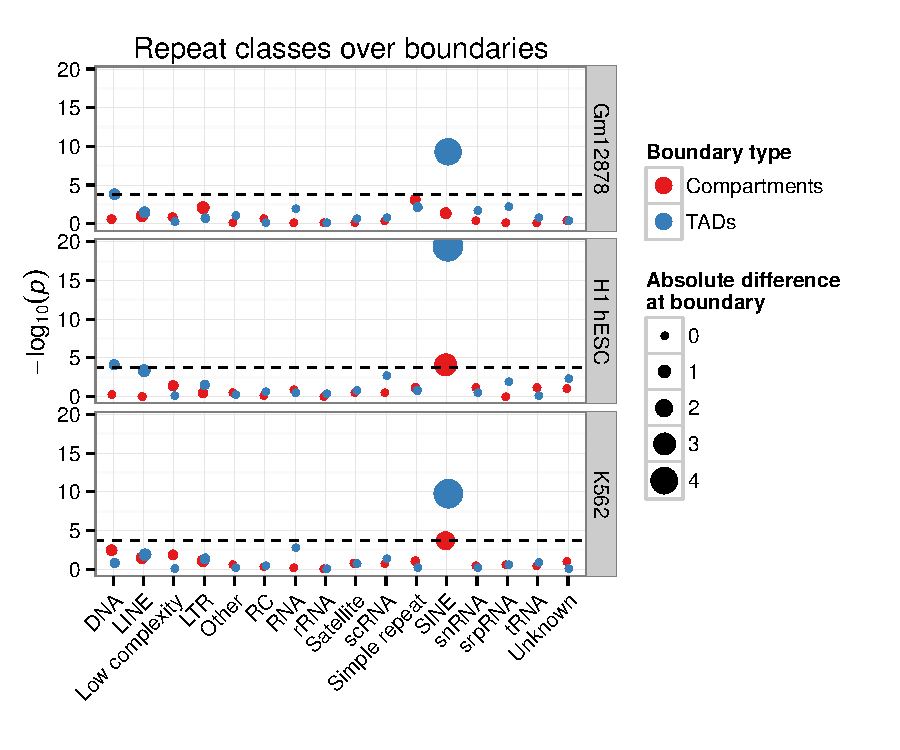
\includegraphics[width=3.2in]{figs/rep_classbubble.pdf}
\captionsetup{width=\textwidth}
\caption[Significance and effect sizes of repeat class enrichments/depletions over boundaries.]{ {\bf Significance and effect sizes of repeat class enrichments/depletions over boundaries.}
Boundary profiles (Fig. \ref{fig:rep_classprofiles}) were tested for enrichment or depletion of each factor at the boundary bin relative to peripheral non-boundary bins (see Methods \ref{boundaries}). Bubble area is proportional to the raw effect size of an enrichment or depletion. The Bonferroni-corrected significance threshold is highlighted with a dashed line.
}\label{fig:rep_classbubble}
\end{center}
\end{figure} 

Repeat class profiles also suggest LINEs may be depleted over TAD boundaries and DNA repeats may be enriched at both boundary types (Fig. \ref{fig:rep_classprofiles}), however statistically these observations do not surpass our pre-defined significance threshold ($\alpha = 0.05$) after multiple testing correction (Fig. \ref{fig:rep_classbubble}).

Repeat classes can be broken into smaller repeat families. \citet{Dixon2012} reported that the Alu (or B1 in mouse) repeat families are enriched over TAD boundaries. Again we can reproduce this finding and extend it to compartment boundaries (Fig. \ref{fig:rep_fambubble}). 

\begin{figure}
\begin{center} 
\makebox[\textwidth][c]{ 
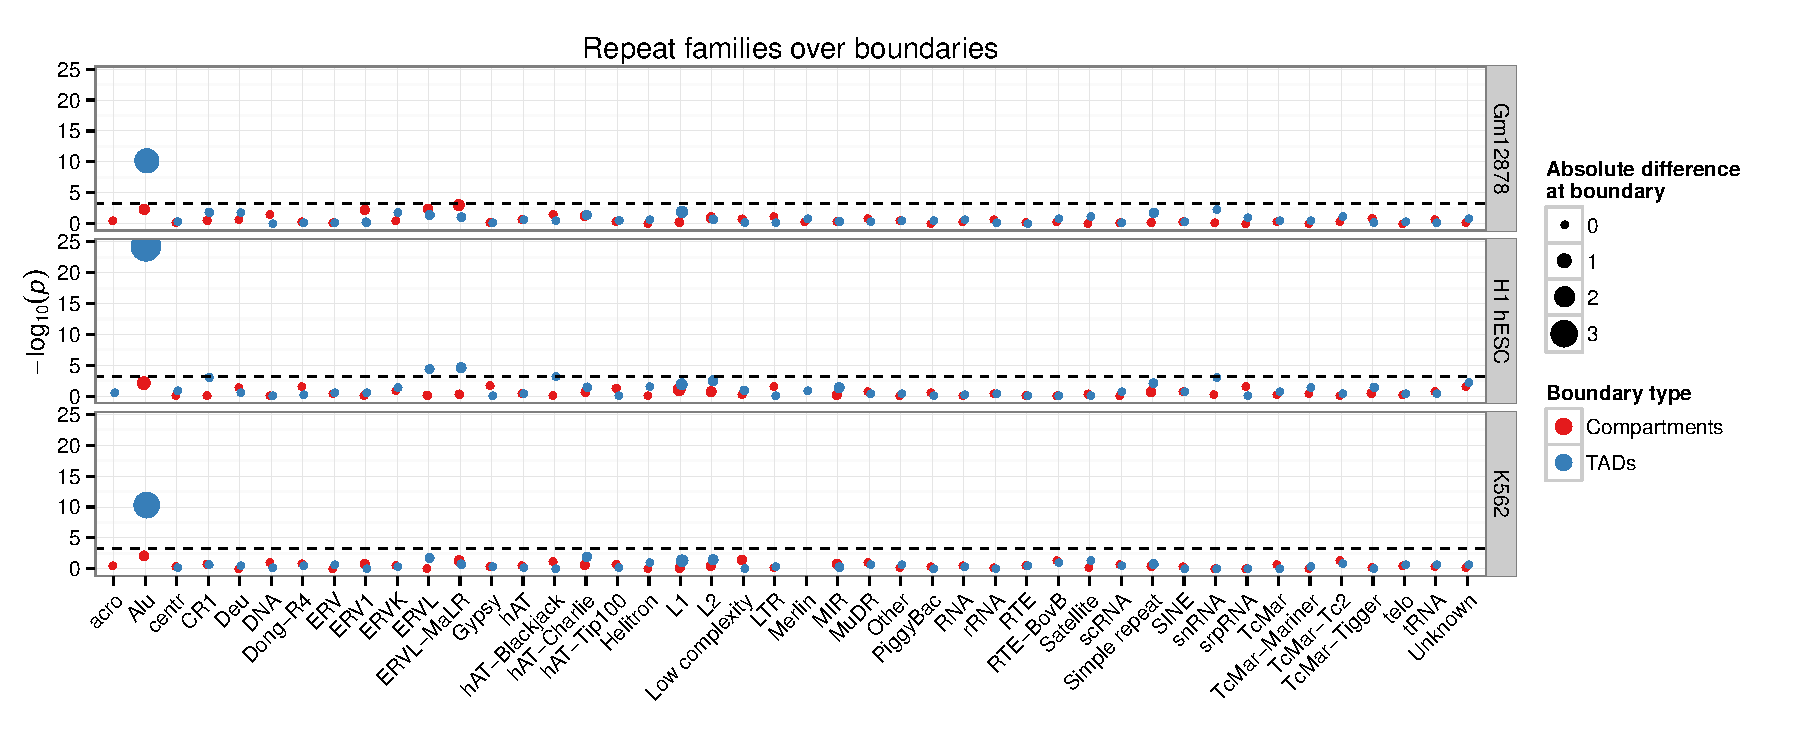
\includegraphics[width=7in]{figs/rep_fambubble.pdf}
}
\captionsetup{width=\textwidth}
\caption[Significance and effect sizes of repeat family enrichments/depletions over boundaries.]{ {\bf Significance and effect sizes of repeat family enrichments/depletions over boundaries.}
As per Fig. \ref{fig:rep_classbubble} but for a higher resolution repeat classification.
}\label{fig:rep_fambubble}
\end{center}
\end{figure} 

% Figure: profiles of those significant + suggestive from all repeat family profiles

\section{De novo boundary prediction}

We have shown TAD and compartment domain boundaries to be well-marked by a variety of features. Compartment boundaries are successfully predicted as a side-effect of modelling the continuous compartment profile eigenvector (Section \ref{sec:modhoc}) however a related measure of activity and repression does not exist for TADs.

We attempted to model TAD boundaries in a variety of ways: firstly a using a class-balanced classification framework and secondly through indirect models of directionality index and the downstream domain-caller HMM state.\cite{Dixon2012}

\subsection{Learning boundary classification}

Results presented in this thesis describe the spectra of chromatin marks over TAD boundaries (Figs. \ref{fig:alltads}, \ref{fig:boundarysummary}), it is thus of interested to test if we can build a predictive model that can call boundary regions from these marks alone. Such a model, if successful, could have broad utility in domain prediction in metazoan organisms where Hi-C data is not available.

A straightforward approach to this modelling task is to build a supervised classifier that learns the associations between two classes of genomic region: those labelled TAD boundaries and those which are not. To this end, we again turn to a Random Forest (RF) model, due to its many attractive properties discussed previously (Methods \ref{sec:rf}). Our input feature set is made up of the same $35$ matched features used in models of compartment eigenvector (Section \ref{sec:modhoc}), with the addition of Alu repeat elements (Section \ref{sec:repeats}). Classifications are those produced by the \citet{Dixon2012} TAD calling algorithm (Methods \ref{meth:tadcalling}), therefore TAD boundaries were resolved to 40 kb bins. We class such bins as boundary true positives (TP), and select matched bins $500$ kb upstream as boundary true negatives (TN) for our training set.

To build parsimonious and accurate models (as discussed in Section \ref{sec:parsimoniousmodels}), we used the \texttt{AUC-RF} algorithm.\cite{Calle2011} This is a form of stepwise model selection which optimises feature subset selection relative to the area under the receiver operating characteristic (AUROC), a metric which captures both the speciality and sensitivity of a classifier. This method was used a training set of $80\%$ of boundaries per cell type, with predictions assessed on out-of-bag (OOB) data as each forest was constructed. Selected models were then applied to the remaining held-out test set of $20\%$ of TAD boundaries, with their matched non-boundary bins (full details are in Methods \ref{meth:tadpred}). 

% AUC-RF optimisation plots
\begin{figure}
\begin{center} 
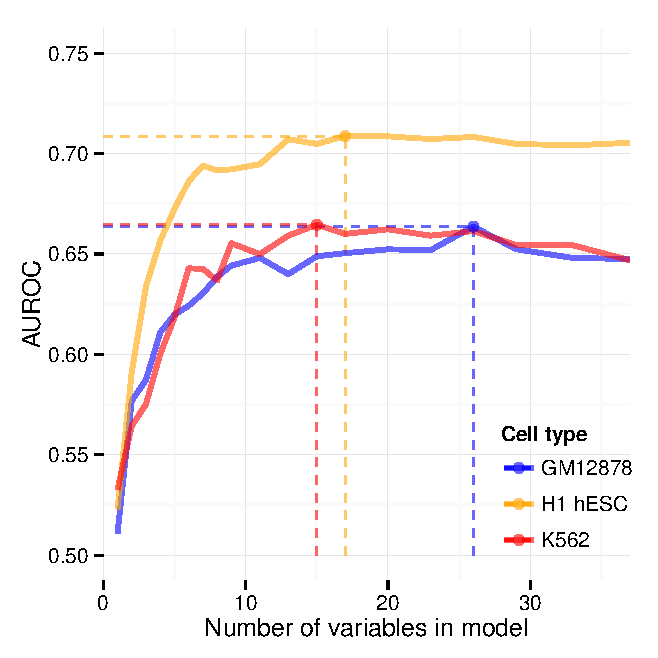
\includegraphics[width=3in]{figs/AUCRF_opt.pdf}
\captionsetup{width=\textwidth}
\caption[ The AUC-RF stepwise algorithm finds that variable subset which maximises the AUROC on out-of-bag data. ]{ {\bf The AUC-RF stepwise algorithm finds that variable subset which maximises the AUROC on out-of-bag data. }
The AUROC is calculated at each stage of a stepwise method for selecting the best subset model from a full featureset. Here AUC-RF selected the following combinations. K562: XXX The AUC-RF algorithm is explained in Methods \ref{meth:tadpred}.
}\label{fig:tadpred_opt}
\end{center}
\end{figure} 


Predictive performance of these models is shown as ROC plus (Fig. \ref{fig:tadpred_auroc}) and in each case an AUROC of around $0.67$--$0.71$ was achieved. In practice, this means that each classifier has around a $70\%$ probability of ranking a random boundary region more highly than a random non-boundary region.\cite{Fawcett2006a} Using a commonly-used AUROC "rule of thumb", this performance falls between the ranges of "poor" to "moderate" classification accuracy.\cite{Streiner2007a}

\begin{figure}
\begin{center} 
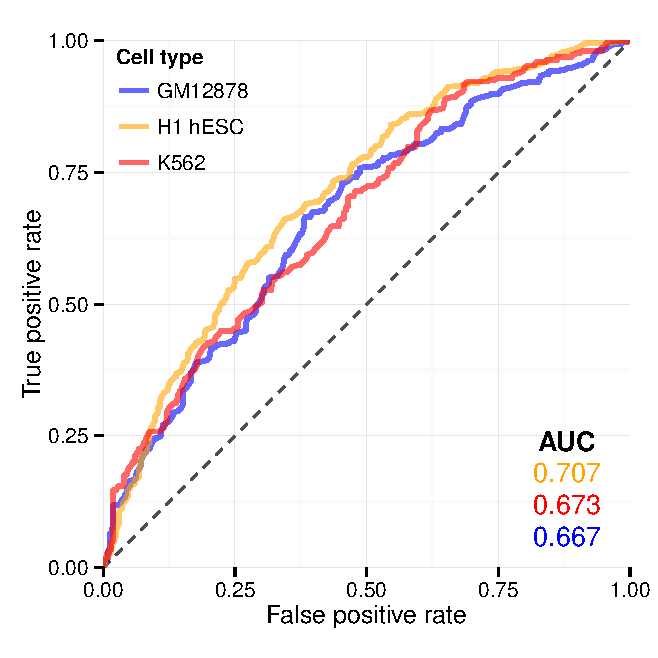
\includegraphics[width=3in]{figs/tadpred_auroc.pdf}
\captionsetup{width=\textwidth}
\caption[ Receiver operating characteristics for TAD boundary classifications. ]{ {\bf Receiver operating characteristics for TAD boundary classifications. }
ROCs are shown for three cell-type specific classifiers of TAD boundary bins. The area under each cure is also shown (\emph{inset}).
}\label{fig:tadpred_auroc}
\end{center}
\end{figure} 

With their moderate-to-low classification accuracy in mind, it is still of interest to analyse the variable importances in each cell type model. We find that CTCF stands out as the most informative variable in each classifier by some margin (Fig. \ref{fig:tadpred_varimp}).

\begin{figure}
\begin{center} 
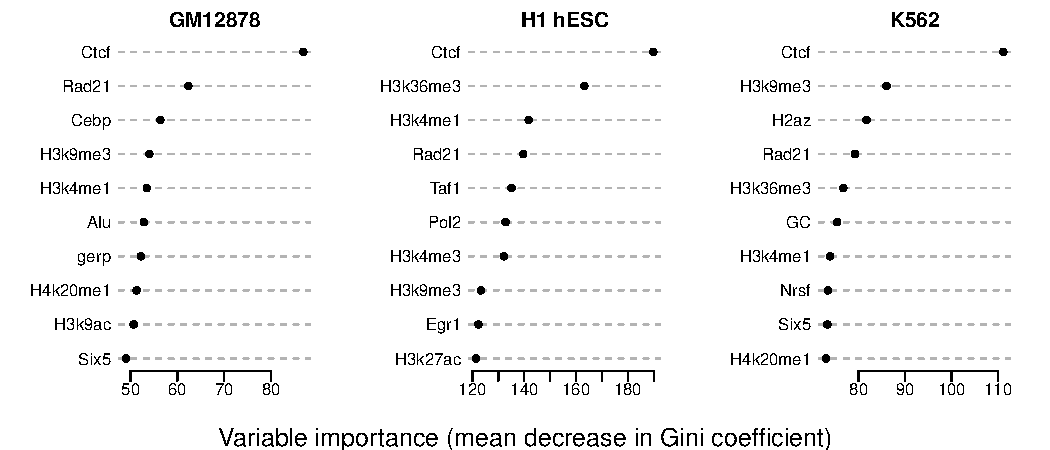
\includegraphics[width=5.45in]{figs/tadpred_varimp.pdf}
\captionsetup{width=\textwidth}
\caption[ Variable importance for boundary classification Random Forest models. ]{ {\bf Variable importance for boundary classification Random Forest models. }
The highest ten most important variables in each boundary classification model are shown and ranked by their variable importance as defined by mean decrease in Gini coefficient when permuted (Methods \ref{meth:tadpred}).
}\label{fig:tadpred_varimp}
\end{center}
\end{figure} 


\section{MetaTAD boundaries}\label{sec:metatads}

Our collaborators uncovered the concept of "metaTADs": sequential aggregations of adjacent and strongly-interacting TADs to form a hierarchy of domain organisation covering each chromosome.

MetaTADs are constructed simply by performing constrained heretical clustering based on inter-TAD contacts. That is, those two neighbour TADs that have the largest number of interTAD contacts are linked to form a metaTAD and this process is recursed until all TADs on a chromosome are joined into a tree-like network which fully describes the hierarchical nature of domain organisation.

My contribution to this work was to explore these newly-described metaTAD structures and perform boundary analysis as was done with TADs and compartments (Section \ref{sec:boundaryenrichments}). A testable hypothesis, for example, is that boundaries of larger metaTAD structures could display greater enrichments for boundary-defining features.

\subsection{MetaTAD / TAD boundary comparison}

Due to the way metaTADs were constructed by our collaborators, by sequential aggregation of TADs (Methods \ref{meth:meta}), boundary comparisons between TADs and metaTADs are not completely straightforward. For one, every metaTAD boundary is, at a lower level, also a TAD boundary hence for a meaningful comparison we compared only a subset of metaTAD boundaries. Selection of this threshold involved a trade-off between maintaining a sufficient sample size of metaTADs and minimising the overlap between metaTAD and TAD boundaries, as a proportion of all TAD boundaries (Fig. \ref{fig:mtcalibrate}).

\begin{figure}
\begin{center} 
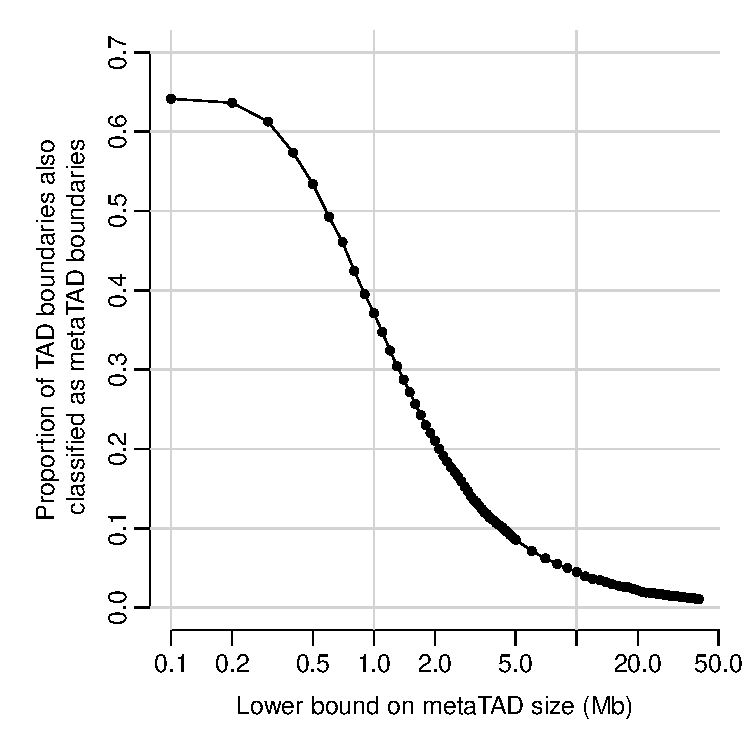
\includegraphics[width=2.75in]{figs/mt_calibrate.pdf}
\captionsetup{width=\textwidth}
\caption[Calibration of metaTAD size selection bounds.]{ {\bf Calibration of metaTAD size selection bounds. }
As the lower bound on metaTAD size is increased, the proportion of all TAD boundaries which are also metaTAD boundaries decreases.
}\label{fig:mtcalibrate}
\end{center}
\end{figure} 

From this calibration plot, a lower bound metaTAD size cut-off of 10 Mb was selected for comparison with TAD boundaries. This left a reasonable sample size of $263$ metaTAD boundaries, while reducing the overlap with the set of all TAD boundaries to approximately $5\%$ (Fig. \ref{fig:mtcalibrate}). We also used an upper bound for size selection, based on observations by our collaborators that interactions between metaTADs larger than around $40$ Mb were no higher than expected background signal (\emph{data not shown}). In practice, almost all boundaries making up metaTADs larger than $10$ Mb are also present in those larger than $40$ Mb, but as hierarchical clustering continued up until a whole chromosome level, this upper bound may exclude a small number of edge-case peripheral TADs which aggregated into chromsome-wide metaTADs without evidence of heightened intra-TAD interactions.

Next a comparison between metaTAD boundaries for metaTAD size ($s$) in the range $10~\textrm{Mb} < s < 40~\textrm{Mb}$ was performed. Our collaborators generated several ChIP-seq datasets, including for CTCF and three PolII variants, as well as expression data in the form of CAGE (Methods \ref{meth:metadata}). We averaged these features over the set of all metaTAD and TAD boundaries and compared the average profiles of each (Fig. \ref{fig:mtfeats}). These average profiles show heightened enrichment for PolII variants, CTCF and DNase, with non-overlapping $95\%$ confidence intervals of the mean over the boundary bin. Increased enrichments of gene density and histone modificationH$3$K$27$me$3$ are also suggestive of a heightened prevalence at metaTAD boundaries relative to TAD boundaries (Fig. \ref{fig:mtfeats}). The observable co-incidence of metaTAD boundaries and lamina associated domains (LADs) is explored further in Section \ref{sec:mtlads}.

\begin{figure}
\begin{center} 
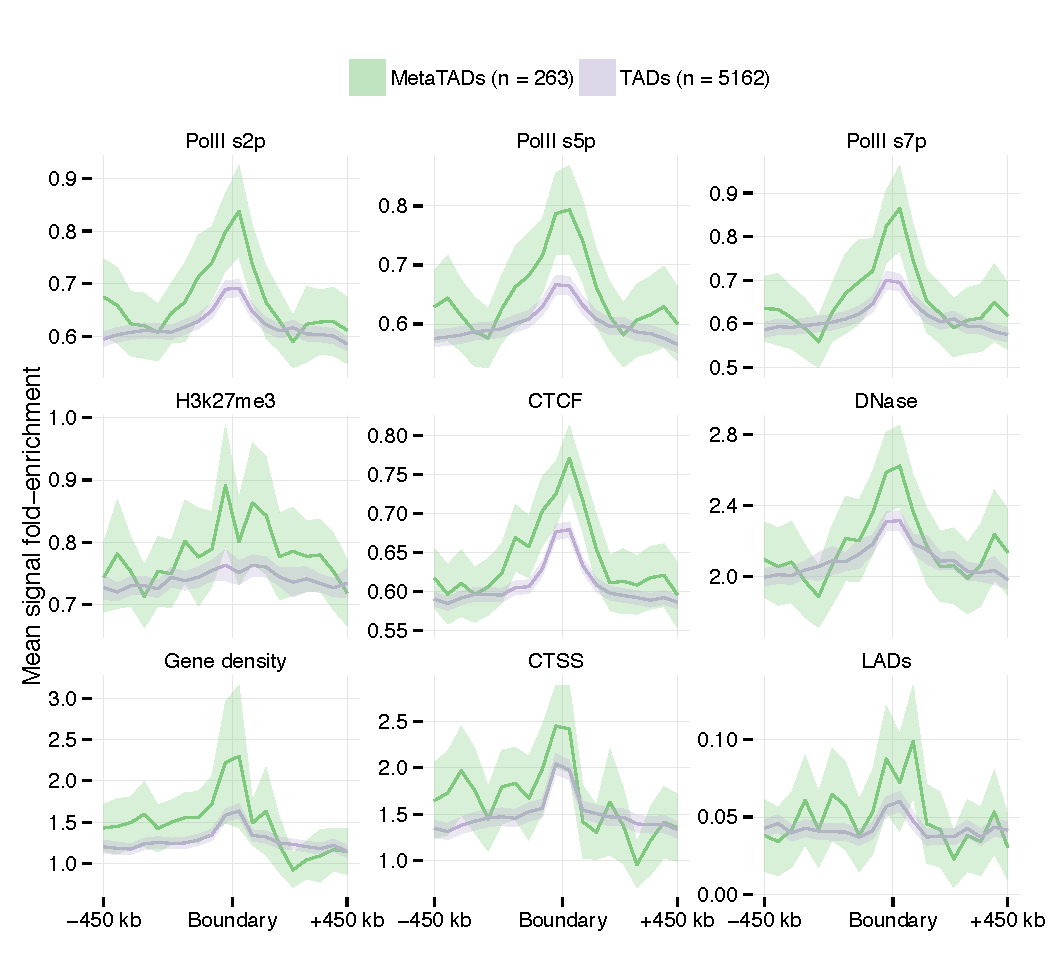
\includegraphics[width=4.5in]{figs/mt_feats.pdf}
\captionsetup{width=\textwidth}
\caption[Large metaTADs show greater enrichments for an array of boundary features.]{ {\bf Large metaTADs show greater enrichments for an array of boundary features.}
Genome-wide profiles of epigenomic features and gene densities averaged over all TAD and metaTAD (10 -- 40 Mb) boundaries (ribbons show $95\%$ confidence intervals of the mean).
}\label{fig:mtfeats}
\end{center}
\end{figure} 

Increased enrichment at metaTAD boundaries relative to TAD boundaries lends evidence to the functional importance of metaTADs, and suggests boundaries become increasingly well-demarcated at higher levels of organisation. However, if this is a genuine biological phenomenon, we'd expect the trend not just to be observable in a comparison between two selected sets, but to increase monotonically as we ascended the metaTAD hierarchy from TADs to chromosomes.

To test this, we reran that above boundary analysis (Fig. \ref{fig:mtfeats}) but at a range of metaTAD size cut-offs (Fig. \ref{fig:mtcutoffenrich}). Generally we find increasing enrichments in metaTAD boundaries relative to TAD bounds through the range of lower bound cutoffs from $0$ to $20$ Mb, possibly with a slight decreased effect size at the highest cutoff of $30$ Mb, where the sample size of boundaries decreases to just $62$ (Fig. \ref{fig:mtcutoffenrich}). This analysis strengthens the evidence for heightened functional enrichment of metaTAD boundaries (Figs. \ref{fig:mtfeats}, \ref{fig:mtcutoffenrich}) and suggests the metaTAD aggregation procedure is capturing boundaries of increasing strength, in terms of enrichment of boundary associated features (e.g. Fig. \ref{fig:alltads}), through the metaTAD hierarchy. 

\begin{figure}
\begin{center} 
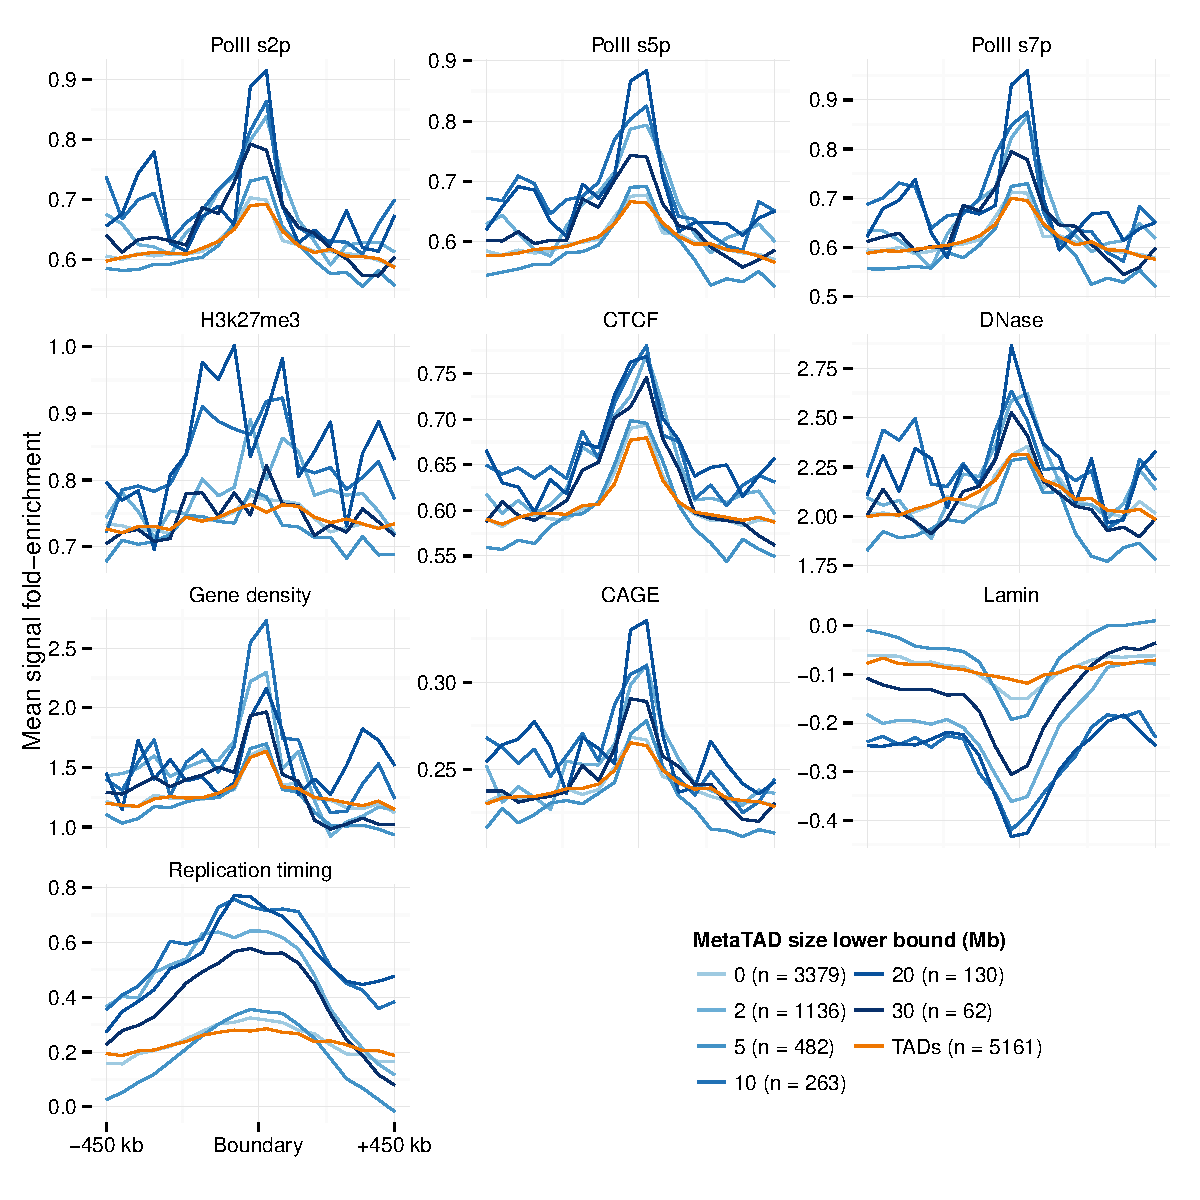
\includegraphics[width=4.5in]{figs/metatad_cutoffenrich.pdf}
\captionsetup{width=\textwidth}
\caption[MetaTADs align with lain associated domains.]{ {\bf MetaTAD boundary enrichments and sample sizes with varying size selection. }
Boundary average-o-grams are shown for TAD and metaTAD boundaries with variable lower bound cut-offs. Sample sizes for each threshold are shown in the legend (\emph{inset}).
}\label{fig:mtcutoffenrich}
\end{center}
\end{figure} 

\subsection{Lamina associated domains}\label{sec:mtlads}

We report a coincidence of metaTAD boundaries and lamina associated domains (LADs), and at a greater level than that observed with smaller TADs (Fig. \ref{fig:mtfeats}). This hints at an association between metaTADs and LADs which can be further investigated.

High resolution LAD data in mouse embryonic stem cells were retrieved from \citet{Peric-Hupkes2010} in the form of continuous measures of lamin-B1 association produced by the DamID technique, known to reflect proximity to the nuclear lamin.\cite{Pickersgill2006} This measure of lamina association was then processed in windows around each metaTAD and TAD boundary, and profiles were combined to form a heatmap (Fig. \ref{fig:mtlamin}).

\begin{figure}
\begin{center} 
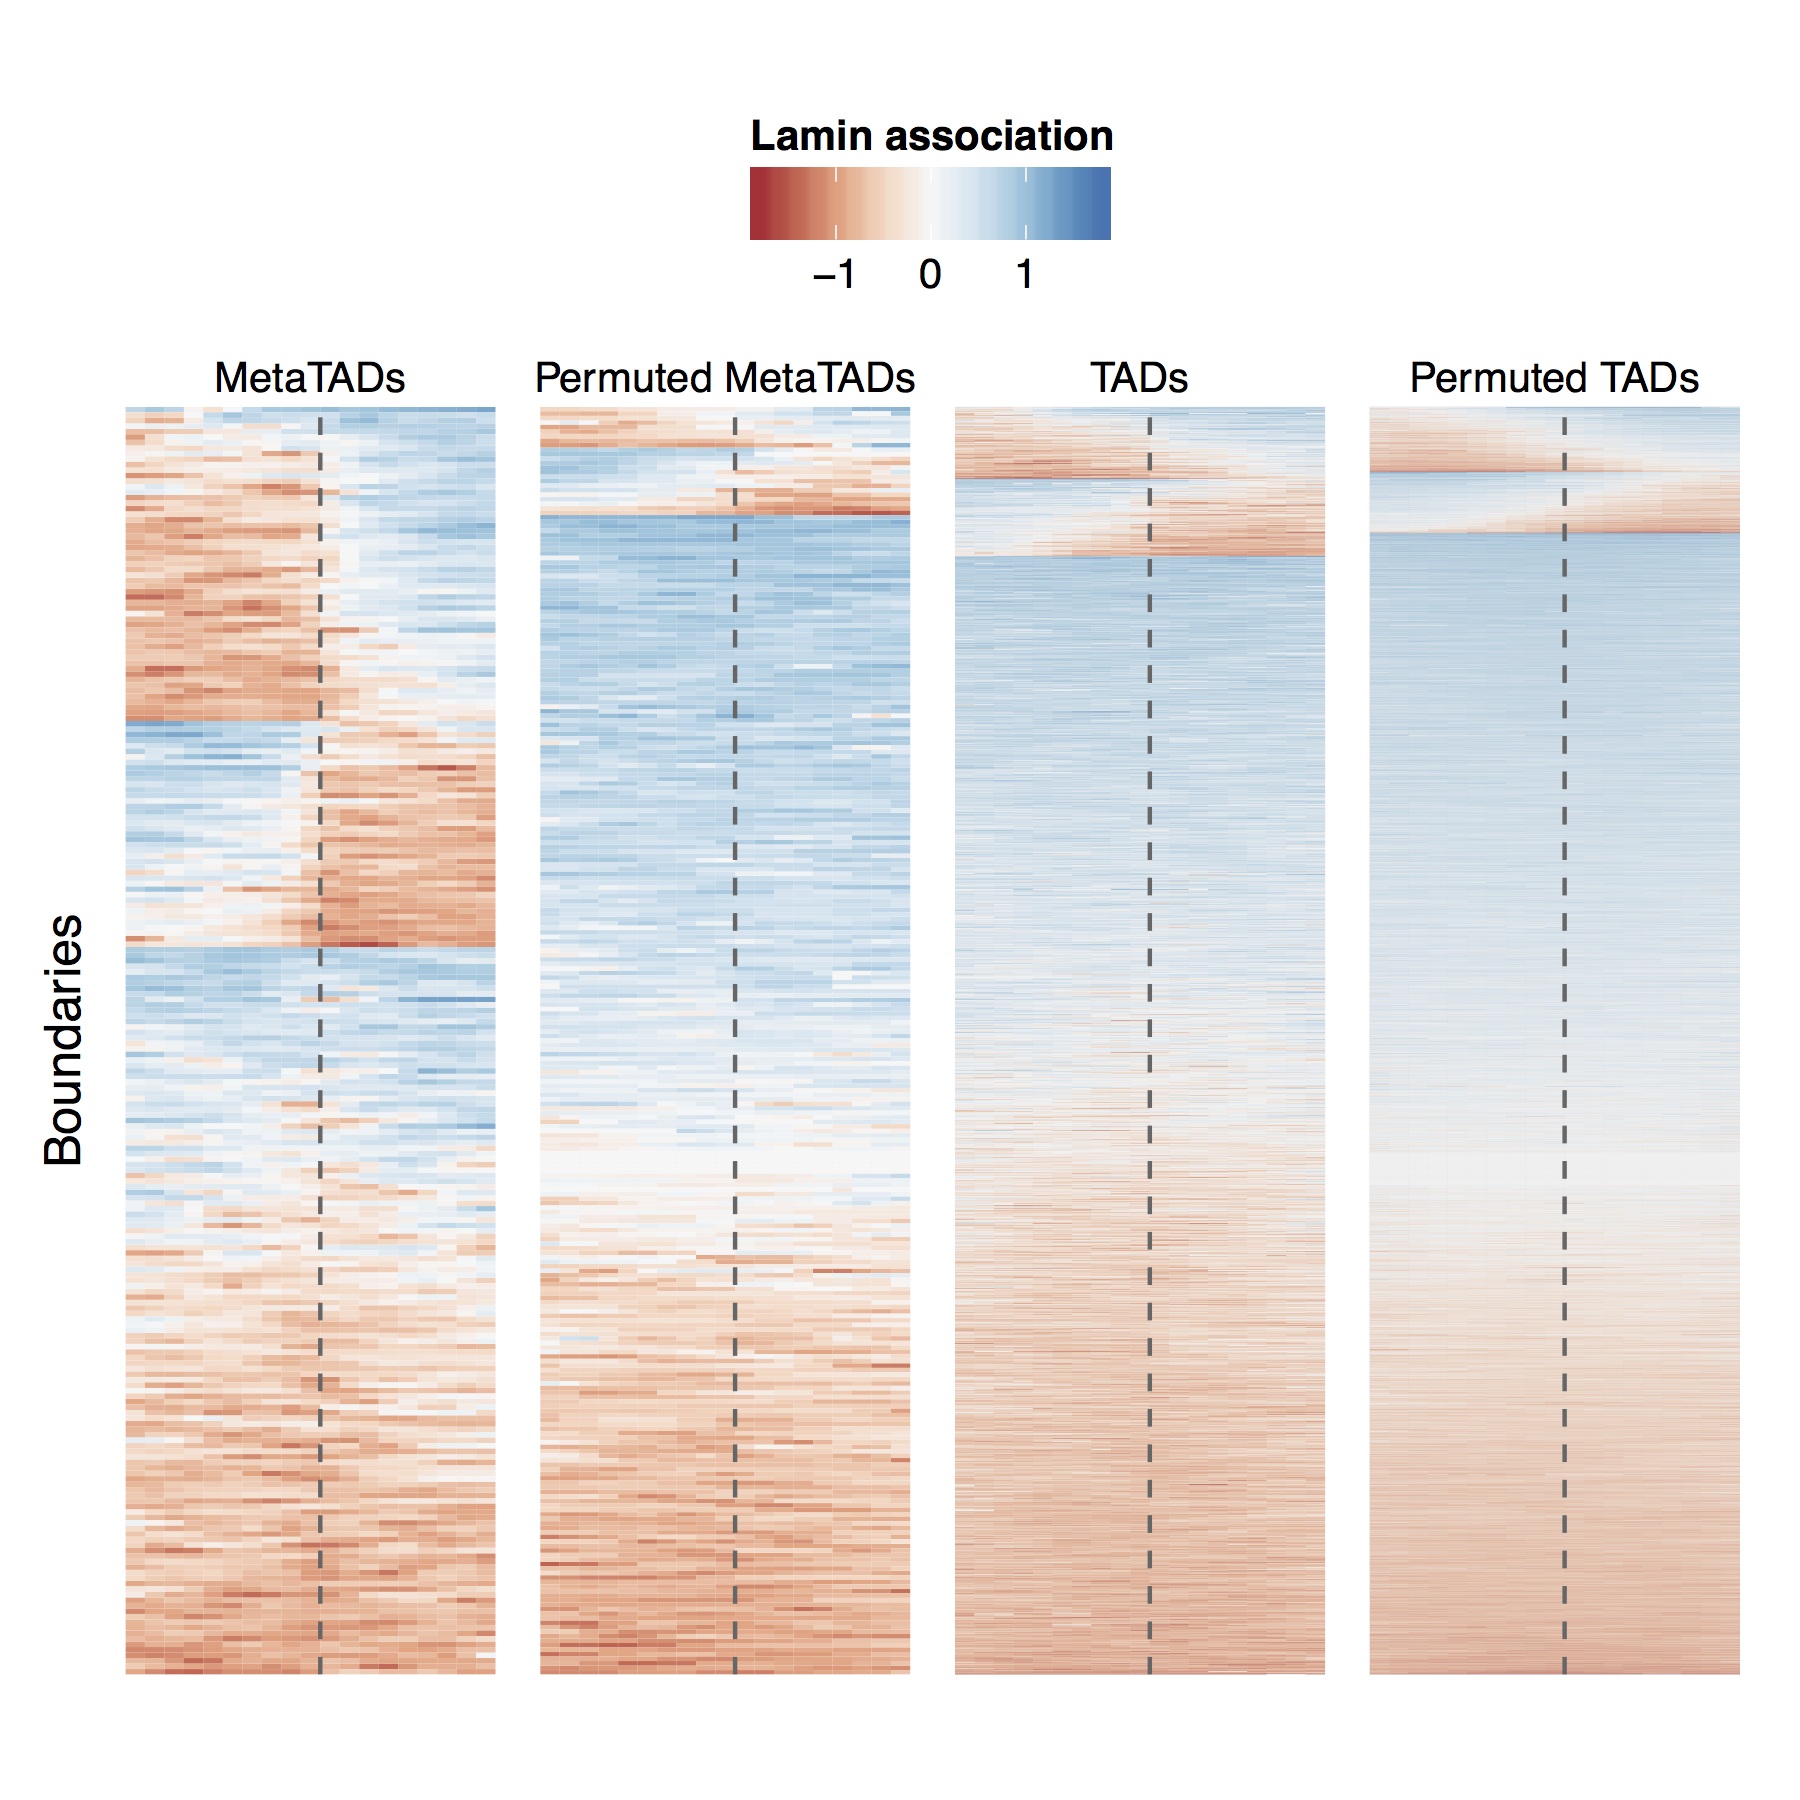
\includegraphics[width=4.5in]{figs/mt_laminperm.png}
\captionsetup{width=\textwidth}
\caption[MetaTADs align with lamin associated domains.]{ {\bf MetaTADs align with lamin associated domains.}
Heatmaps of LaminB1 association microarray probe intensity values over MetaTAD boundaries (from domains of size 10 -- 40 Mb) and TAD boundaries, are displayed alongside examples of circularly-permuted boundaries. Profiles are shown $\pm450$ kb from each boundary.
}\label{fig:mtlamin}
\end{center}
\end{figure} 

Boundaries were seriated in order to separate out those that coincide with a LAD boundary (Methods \ref{meth:metalad}) and we found a large number of metaTAD boundaries ($43\%$) in our $10$--$40$ Mb subset appeared to correspond to LAD boundaries (Fig. \ref{fig:mtlamin}). The same comparison using TAD boundaries found a coincidence of just $12\%$. However LADs are large domains and there were over $5,000$ TADs called in this Hi-C data by our collaborators, thus in absolute numbers of boundaries this is still represents a large overlap.

To test the significance of these observations, we apply a permutation-based statistical test where our observed coincidences are compared with those produced by $1,000$ circular (per-chromosome) permutations (Methods \ref{meth:metalad}). We found that the metaTAD boundary coincidence is around $2.7$-fold increase above null expectation (observed: $42.6\%$; expected: $15.8\%$; empirical $p$-value: $p < 1 \times 10^{-4}$; Fig. \ref{fig:mtsummary}). Meanwhile TAD boundaries were found to have a smaller, yet still significant, $1.2$-fold increase in coincidence with LAD boundaries relative to a null model (observed: $11.8\%$; expected: $9.5\%$; empirical $p$-value: $p < 1 \times 10^{-4}$; Fig. \ref{fig:mtsummary}).

\begin{figure}
\begin{center} 
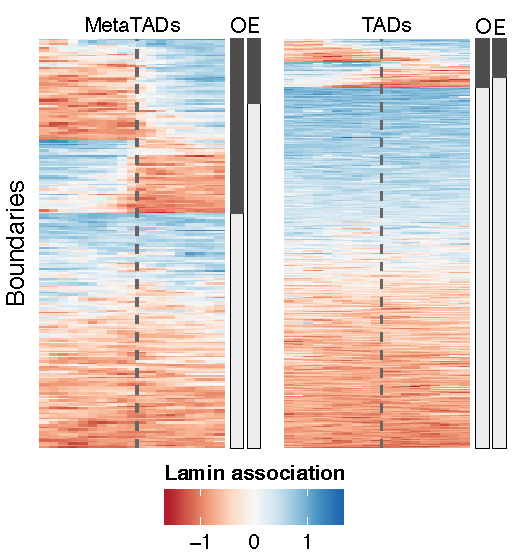
\includegraphics[width=2.5in]{figs/mt_laminsummary.pdf}
\captionsetup{width=\textwidth}
\caption[ MetaTAD boundaries much LAD boundaries much more often than expected by chance. ]{ {\bf MetaTAD boundaries much LAD boundaries much more often than expected by chance. }
Heatmaps of lamina association over MetaTAD boundaries are shown as in Fig. \ref{fig:mtlamin}. Sidebars labelled O and E reflect observed and expected proportions of metaTAD / LAD boundary overlaps.
}\label{fig:mtsummary}
\end{center}
\end{figure} 

This result highlights again that metaTADs offer useful perspectives onto higher order genome organisation. In this case, it appears TADs will often neatly aggregate within LADs and together these constitute what we observe as a metaTAD.

\subsection{Boundaries over a time series}

For the first time, our collaborator's applied the Hi-C technique over a differentiation time course from mouse embryonic stem cells, to neural pre-cursors and finally fully-differentiated neuron cells. Successive expression measures were also taken alongside this Hi-C data in the form of CAGE data, produced by the FANTOM5 consortium.\cite{fantom5} Together these datasets offer a unique perspective onto how higher order genome organisation varies with expression during differentiation. 

Collaborators explored changes in both the overall tree structure between timepoints, and aggregate expression changes between TADs and metaTADs at successive timepoints. They identified rewiring events in the metaTAD tree over the timecourse, and found corresponding changes in expression (\emph{data not shown}). Given metaTAD structures appear to differ and matched CAGE data exists for each timepoint, it was of interest to test how observed boundary enrichments for gene expression (Figs. \ref{fig:mtfeats}, \ref{fig:mtcutoffenrich}) might vary over this timecourse. 

\begin{figure}
\begin{center} 
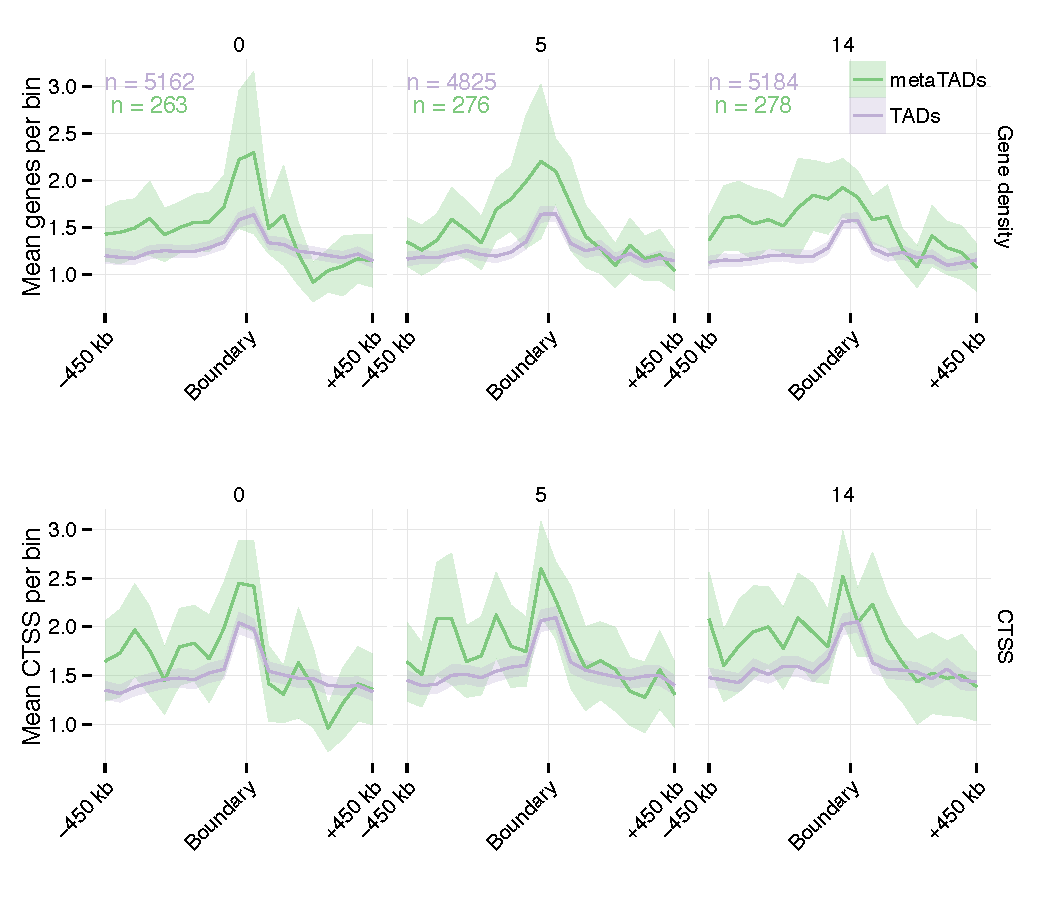
\includegraphics[width=4.5in]{figs/mt_ts.pdf}
\captionsetup{width=\textwidth}
\caption[Observed enrichments persist over a time series.]{ {\bf Observed enrichments persist over a time series.}
CAGE-defined active TSS (CTSS) were counted per $50$ kb bin across each TAD and MetaTAD ($10$--$40$ Mb) boundary and averaged (ribbons show $95\%$ confidence intervals of the mean). Gene densities refer to mean counts of annotated genes per bin, with an overlap of at least 250 bp.
}\label{fig:mtts}
\end{center}
\end{figure} 

We find actively-transcribed CAGE-defined TSS (CTSS) to be consistently enriched over the shifting boundaries through the differentiation timecourse (Fig. \ref{fig:mtts}). We coupled this with a static measure of gene density in order to distinguish expression changes from genic overlap, however both series show similar patterns so it does not seem that boundary expression changes occur at a global scale over this timecourse. Peak heights over boundary bins suggest modestly stronger enrichments at metaTAD boundaries relative to TAD boundaries, as seen with other features (Fig. \ref{fig:mtfeats}). 

\section{Other boundaries}

\subsection{Giemsa bands}

% text (colin's?) from pre-submission old manuscript draft
A recent analysis of Hi-C datasets examined the hierarchy of nuclear compartment and TAD organisation in human HeLa cells across the cell cycle. They found that interphase and metaphase chromatin structure are highly distinct, such that the TADs and compartments observed here are effectively abolished in metaphase.\cite{Naumova2013} This raises the question of how the structural organization seen in (and often shared between) interphase cells is inherited through the cell cycle.

Human Giemsa metaphase banding (G-band) pattern data have been integrated with the human genome assembly, and although such data are widely used, they are also necessarily of low resolution.\cite{Furey2003} These G-band patterns are constant over human cell types at metaphase, but all traces of interphase higher order structure were reported to be absent at metaphase.\cite{Naumova2013} We would therefore expect no agreement between metaphase G-bands and the patterns of interphase TADs and A/B nuclear compartments defined here, over all three cell types. 

We examined the genome wide similarity of all interphase domain structure boundaries to metaphase G-band boundaries, relative to an expected distribution derived by permutation (Methods \ref{giemsa-band-comparison}). There is a significant, though modest, excess of compartment boundaries within close proximity of G-band boundaries, such that $13.90\%$ of compartment boundaries are within $500$ kb of a G-band boundary (expectation = $10.50\%$, K-S test: D $= 0.076$, p $< 3 \times10^{-12}$). This is seen for compartment boundaries calculated for all three cell types independently (a full comparison for GM12878 is shown in Fig. \ref{fig:gbands2}). 

\begin{figure}
\begin{center} 
\makebox[\textwidth][c]{ 
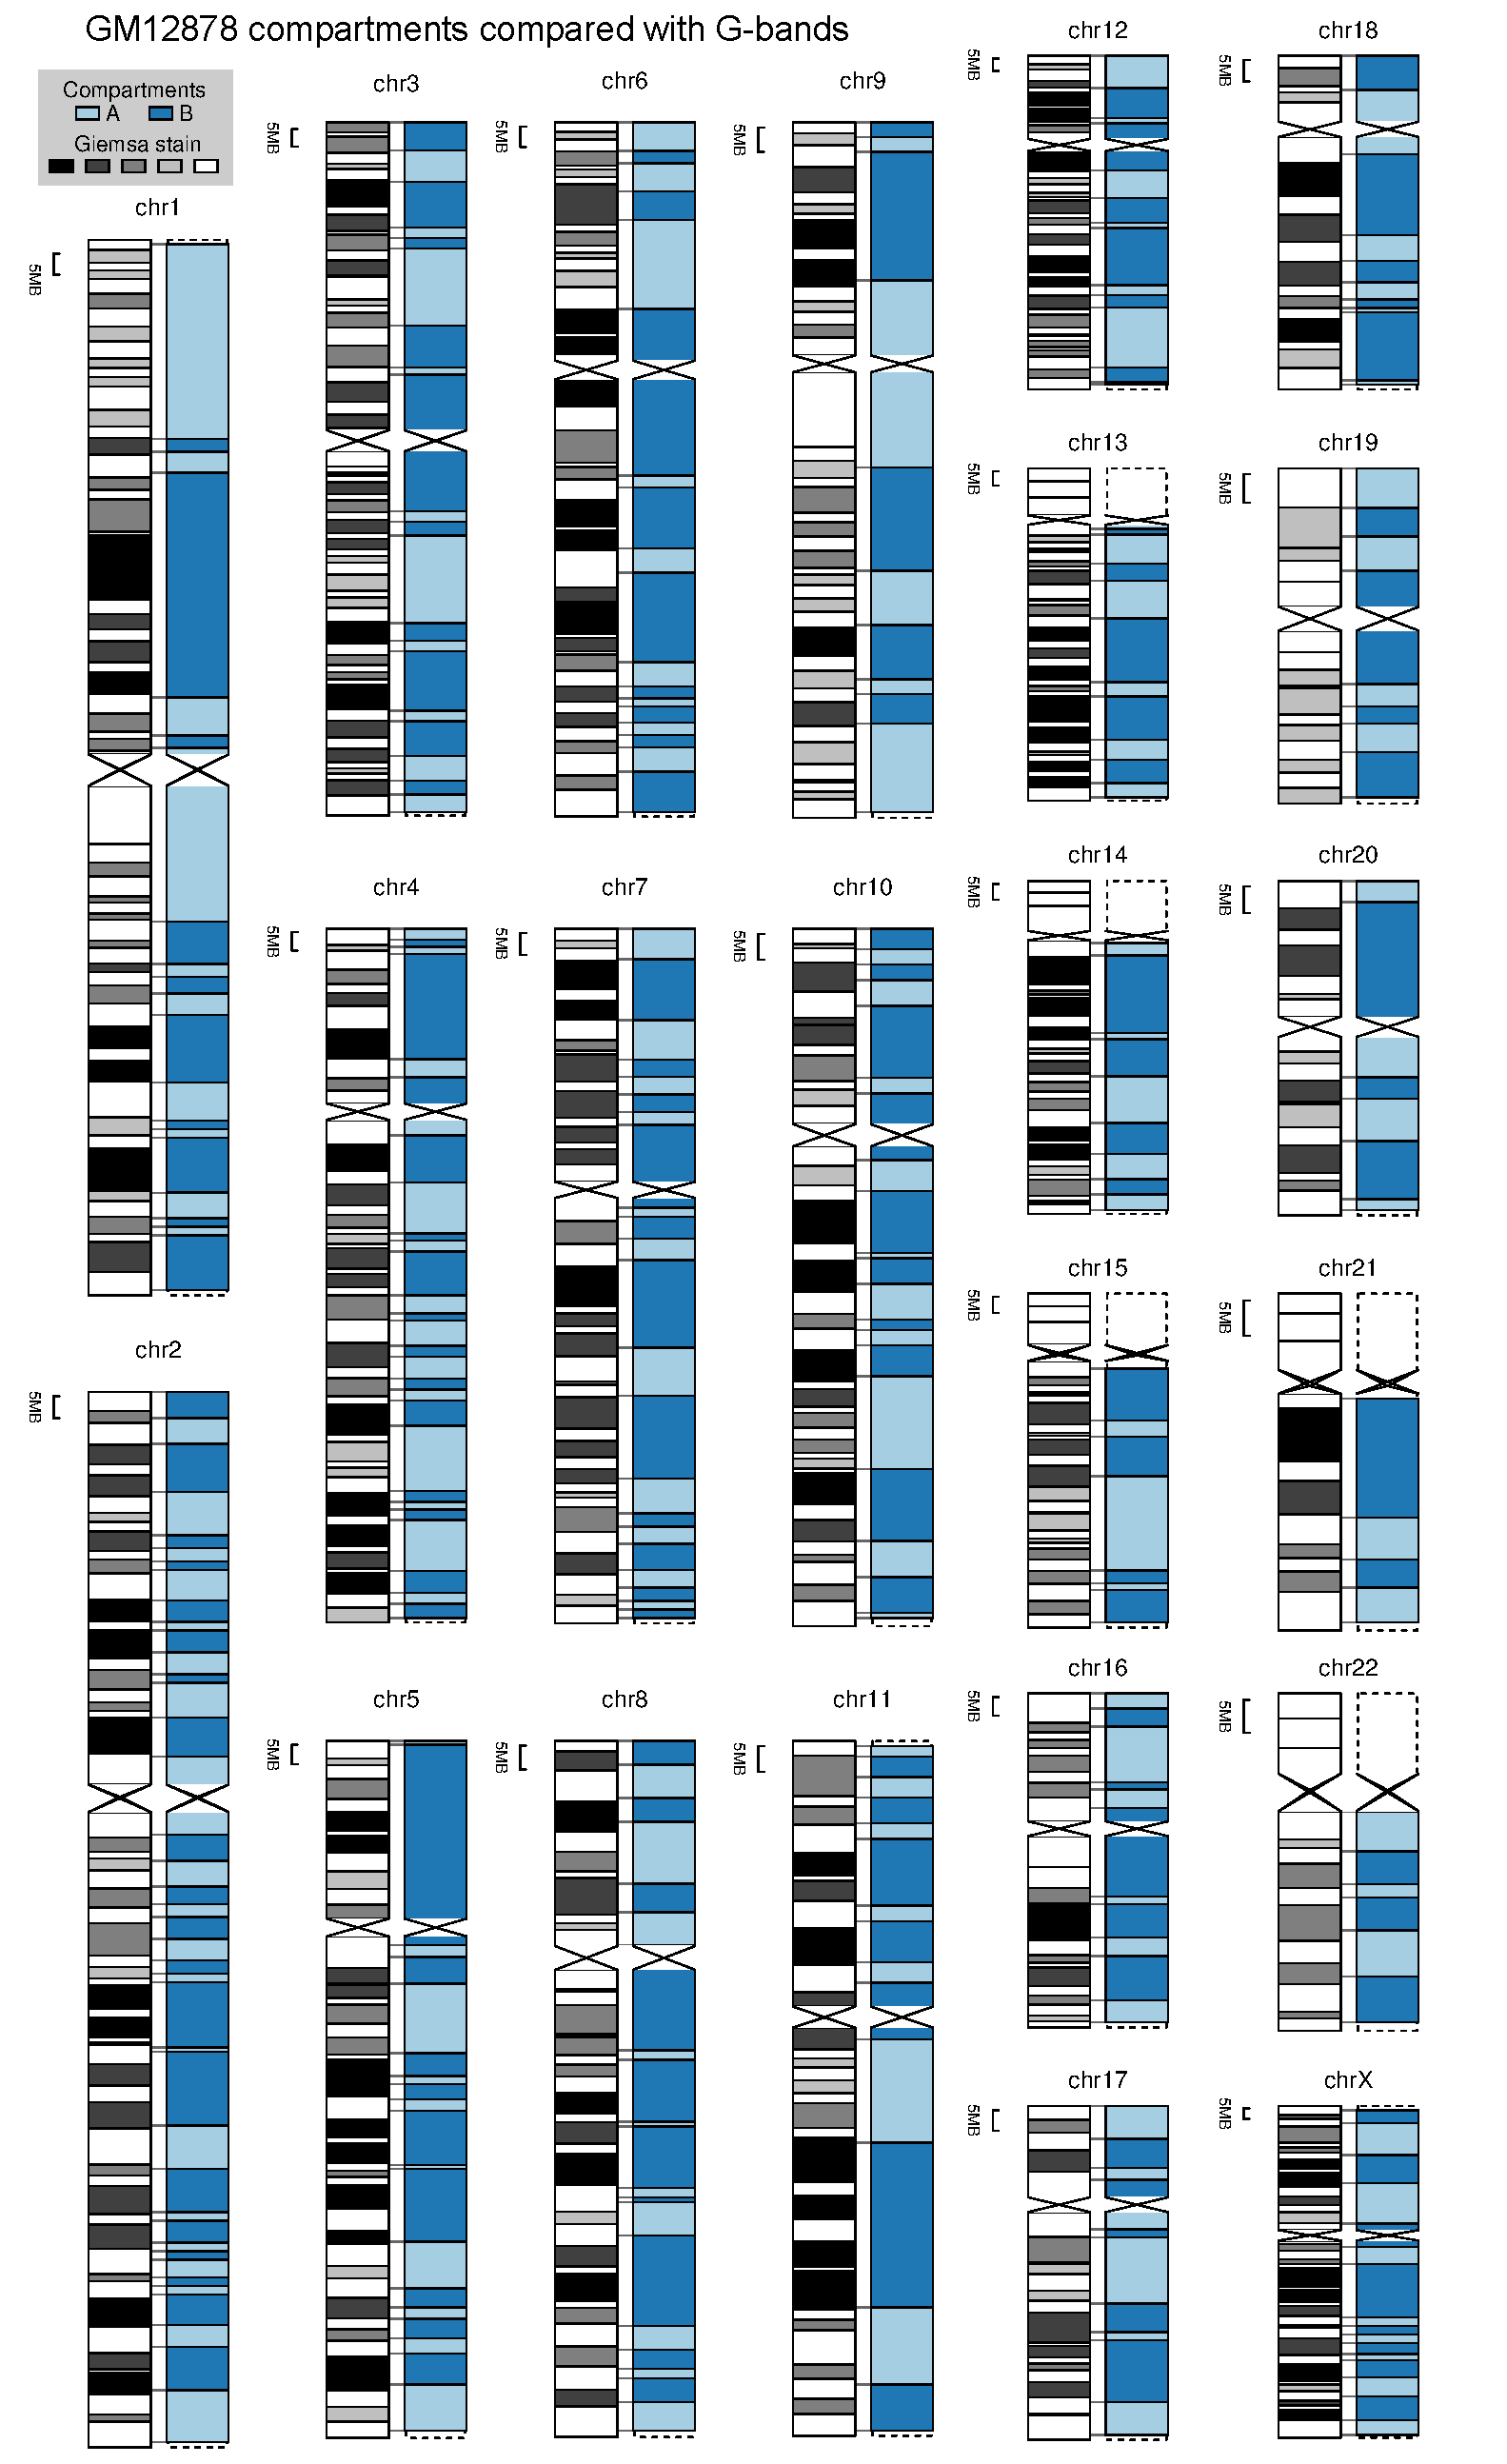
\includegraphics[width=5.7in]{figs/gb_ideo.pdf}
}
\captionsetup{width=\textwidth}
\caption[Genome-wide agreement between Giemsa bands and A/B compartments..]{ {\bf Genome-wide agreement between Giemsa bands and A/B compartments. }
G-bands, assayed at metaphase, often correspond with interphase A/B compartments across all chromosomes. Data for cell type GM$12878$ is shown.
}\label{fig:gbands2}
\end{center}
\end{figure} 

The genome wide overlap of compartment A and B regions with particular G-band classes is nonrandom, and suggests much greater correspondence. Regions assigned to compartment A are significantly over-represented within lighter staining (especially G-negative) bands, while compartment B regions are over-represented in the most darkly staining (G-positive) bands (Fig. \ref{fig:gbands}). Approximately $40\%$ of the genome jointly occupies interphase compartment A as well as gneg/gpos25 metaphase G-bands, or occupies the interphase B compartment as well as gpos75/gpos100 at metaphase. Again, the same trends are seen significantly across all three cell types. This agreement is not unexpected given the broad differences in G-negative and G-positive bands, with contrasting gene density, GC content and replication timing\cite{Furey2003} that is strongly reminiscent of the contrasts between interphase A and B compartments,\cite{Lieberman2009} but to our knowledge has not been directly studied before. These data suggest that across the genome most fine structure, reflected in domain boundaries, is not well preserved between interphase and metaphase. However there is evidence for conservation of broader structural categories across a substantial fraction of the genome, which may reflect broad similarities in the degree of compaction seen at many regions across the cell cycle.

\begin{figure}
\begin{center} 
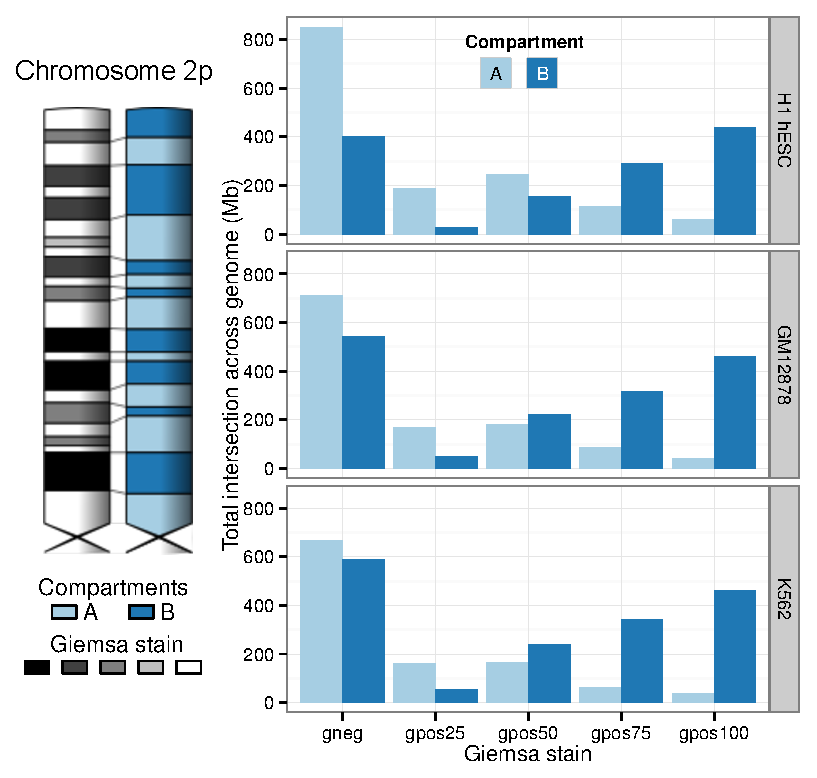
\includegraphics[width=3.8in]{figs/gbands.pdf}
\captionsetup{width=\textwidth}
\caption[ Giemsa--stain bands correspond to A/B compartments.]{ {\bf Giemsa--stain bands correspond to A/B compartments.}
The correspondence between G-bands and A/B compartments is broken down into the five levels of Giemsa stain. A compartments largely match \emph{gneg} staining, while \emph{gpos75} and \emph{gpos100} are enriched in B compartments.
}\label{fig:gbands}
\end{center}
\end{figure} 

%\subsection{Superboundaries}
%
%Thus far compartment and TAD boundaries have been considered separately, however it is of interest to consider how these boundary regions interact across scales. Open questions remain about the co-occurence of these two boundary regions, and whether 


\ifstandalone
\begin{small}
\bibliography{/Users/benmoore/Documents/library,/Users/benmoore/Documents/customrefs}
\end{small}
\fi

\end{document}
